\documentclass[10pt,a4paper,twoside]{book}

%include the configuration file for layout
%Have a look in this file it has some useful commands defined
\usepackage{setspace}
\usepackage{geometry}
\usepackage[toc,page]{appendix}
\usepackage{lipsum}
\usepackage[export]{adjustbox}
\usepackage[T1]{fontenc}
\usepackage{textcomp}
\usepackage{epsfig,graphics}
\usepackage{graphicx}
\usepackage{titlesec}


%%%%%%%%%%%%%%%%%%%%%%%%%%%%%%%%%%%%%%%%%%%%%%%%%%%%%%%%%%%%%%%%%%%%%%%%%%%%%%
% Details of your dissertation
%%%%%%%%%%%%%%%%%%%%%%%%%%%%%%%%%%%%%%%%%%%%%%%%%%%%%%%%%%%%%%%%%%%%%%%%%%%%%%
\newcommand{\projectTitle}{Vive Virtual Reality Technology Demonstration}
\newcommand{\fullname}{Khen Cruzat and Philip Nilsson}
\newcommand{\degreeTitle}{Computer Science}
\newcommand{\session}{2016/2017}

%%%%%%%%%%%%%%%%%%%%%%%%%%%%%%%%%%%%%%%%%%%%%%%%%%%%%%%%%%%%%%%%%%%%%%%%%%%%%%
% Change the geometry of the page to have a 25 mm binding edge
%%%%%%%%%%%%%%%%%%%%%%%%%%%%%%%%%%%%%%%%%%%%%%%%%%%%%%%%%%%%%%%%%%%%%%%%%%%%%%
 \geometry{
 a4paper,
 total={210mm,297mm},
 left=25mm,
 right=25mm,
 top=25mm,
 bottom=20mm,
 }
 
%%%%%%%%%%%%%%%%%%%%%%%%%%%%%%%%%%%%%%%%%%%%%%%%%%%%%%%%%%%%%%%%%%%%%%%%%%%%%%
% Commands to set the line spacing
%%%%%%%%%%%%%%%%%%%%%%%%%%%%%%%%%%%%%%%%%%%%%%%%%%%%%%%%%%%%%%%%%%%%%%%%%%%%%%
 %\singlespacing
 \onehalfspacing
 %\doublespacing
 
%%%%%%%%%%%%%%%%%%%%%%%%%%%%%%%%%%%%%%%%%%%%%%%%%%%%%%%%%%%%%%%%%%%%%%%%%%%%%%
% Spacing for the chapter header
%%%%%%%%%%%%%%%%%%%%%%%%%%%%%%%%%%%%%%%%%%%%%%%%%%%%%%%%%%%%%%%%%%%%%%%%%%%%%%
 \titleformat{\chapter}[display]
    {\normalfont\Huge\bfseries}{\vspace*{-1\baselineskip}\chaptertitlename\ \thechapter}{15pt}{\huge}
\titlespacing*{\chapter}{0pt}{0pt}{15pt}

\renewcommand\bibname{References}

%%%%%%%%%%%%%%%%%%%%%%%%%%%%%%%%%%%%%%%%%%%%%%%%%%%%%%%%%%%%%%%%%%%%%%%%%%%%%%
% Some shortcuts that maybe useful
%%%%%%%%%%%%%%%%%%%%%%%%%%%%%%%%%%%%%%%%%%%%%%%%%%%%%%%%%%%%%%%%%%%%%%%%%%%%%%
\DeclareTextCommandDefault{\textcopyright}{\textcircled{c}}
 
%%%%%%%%%%%%%%%%%%%%%%%%%%%%%%%%%%%%%%%%%%%%%%%%%%%%%%%%%%%%%%%%%%%%%%%%%%%%%%
% Bibliography style: choose one and make sure you have the relevant .bst file
%%%%%%%%%%%%%%%%%%%%%%%%%%%%%%%%%%%%%%%%%%%%%%%%%%%%%%%%%%%%%%%%%%%%%%%%%%%%%%
\bibliographystyle{abbrv}


%%%%%%%%%%%%%%%%%%%%%%%%%%%%%%%%%%%%%%%%%%%%%%%%%%%%%%%%%%%%%%%%%%%%%%%%%%%%%%
% Layout for the front cover !!!!! YOU SHOULD NOT HAVE TO CHANGE THIS!!!!!
%%%%%%%%%%%%%%%%%%%%%%%%%%%%%%%%%%%%%%%%%%%%%%%%%%%%%%%%%%%%%%%%%%%%%%%%%%%%%%
 
\newcommand{\frontcover}{
% The title page:
\begin{titlepage}
\newgeometry{left=25mm,right=25mm,top=45mm,bottom=0.1cm}

\begin{minipage}[t]{7cm}
\noindent\textbf{\Large{School of Computing}}\\
{\fontfamily{ptm}\selectfont 
\uppercase{faculty of engineering}
}
\end{minipage}
\hfill
\begin{minipage}[t]{7cm}
\vspace*{-25pt}

\includegraphics[scale=0.2,right]{logo_black.png}
\vspace*{-1pt}
\end{minipage}

\noindent\makebox[\linewidth]{\rule{\paperwidth}{0.4pt}}

\centering
\vspace*{37mm}
\textbf{\Large\projectTitle}\\
\vspace*{10mm}
\textbf{\large\fullname}\\
\vspace*{10mm}
\textbf{Submitted in accordance with the requirements for the degree of}\\
\textbf{\degreeTitle}\\
\vspace*{10mm}
\session\\
\restoregeometry
\end{titlepage}
}

%%%%%%%%%%%%%%%%%%%%%%%%%%%%%%%%%%%%%%%%%%%%%%%%%%%%%%%%%%%%%%%%%%%%%%%%%%%%%%
% Define a new environment for the dissertation summary
%%%%%%%%%%%%%%%%%%%%%%%%%%%%%%%%%%%%%%%%%%%%%%%%%%%%%%%%%%%%%%%%%%%%%%%%%%%%%%
\newenvironment{dissertationsummary}
 	{\cleardoublepage \null 
 		\begin{center}%
			\textbf{Summary}
		\end{center}}%
	{\vfill \null }



\begin{document}
%The prelude is everything upto the start of chapter 1
\pagenumbering{roman}
\frontcover

\clearpage
\noindent The candidate confirms that the following have been submitted.\\
<As an example>
\begin{table}[ht!]
\begin{tabular}{|p{0.3\textwidth}|p{0.3\textwidth}|p{0.3\textwidth}|}
\hline 
Items & Format & Recipient(s) and Date \\ 
\hline 
Final Report (2 copies) & Report & SSO (DD/MM/YY) \\ 
\hline 
Final Report (digital) & Report & VLE (DD/MM/YY) \\ 
\hline 
Project Code & GitHub Repository & Supervisor, Assessor (DD/MM/YY) \\ 
\hline 
User Manual & Report Appendix & Client, Supervisor (DD/MM/YY) \\ 
\hline 
\end{tabular} 
\end{table}

\noindent Type of project: Software Product
\vspace{\fill}\\
\noindent The candidate confirms that the work submitted is their own and the appropriate credit has been given where reference has been made to the work of others.
\vspace{\fill}\\
\noindent I understand that failure to attribute material which is obtained from another source may be considered as plagiarism.
\vspace{\fill}\\
% \flushright(Signature of Student) \rule{50mm}{1pt}
% \flushleft \rule{50mm}{1pt}
\begin{tabular}[t]{@{}l} 
  \rule{50mm}{1pt}\\  Khen Cruzat
\end{tabular}
\hfill% move it to the right
\begin{tabular}[t]{l@{}}
   \rule{50mm}{1pt}\\ Philip Nilsson
\end{tabular}
\flushleft 
\vspace{\fill}
\textcopyright~\session~The University of Leeds and~\fullname
% Summary

\begin{dissertationsummary}
Virtual reality is cutting-edge technology where many industries are becoming interested in. The potential which virtual reality can bring to current lifestyles both in work and entertainment has helped in the boost of development for higher end virtual reality platforms. The University of Leeds regularly holes open days where prospective students come to the university and explore the many possibilities that the university has in store. The School of Computing at University of Leeds currently uses off the shelf software  with the current best virtual reality solution for consumers called HTC Vive. The problem that this project aims to solve is that the School of Computing requires a software that demonstrates computer science skills to create which takes advantage of virtual reality hardware.
\end{dissertationsummary}

\clearpage
\centering\textbf{Acknowledgements}
\flushleft
We would like to thanks both Dr. Hamish Carr and Dr. Andy Bulpitt for all the guidance and advice they have provided to us throughout the project. Weekly meetings and thorough planning sessions were helpful towards the success of this project. The meetings inspired motivation and time to reflect on current progress on the project and an opportunity to discuss challenges faced.
\newline
\par
We would also like to thank the School of Computing support staff especially Judi Drew for their help in granting access to the development room. They enabled us to work on the project whenever work was needed to be done.

% The contents
\tableofcontents

% The list of figures and tables Uncomments the 3 following lines
%to see a list of tables and list of figures.
%\clearpage
%\listoffigures
%\listoftables

%include as many chapters as you have.
%the chapters are in a directory called Chapters
\chapter{Introduction}
\label{chapter1}

%%%%%%%%%%%%%%%%%%%%%%%%%%%%%%%%%%%%%%%%%%%%%%%%%%%%%%%%%%%%%%%%%%%%%%%%%%%%%%
% Project Statement
%%%%%%%%%%%%%%%%%%%%%%%%%%%%%%%%%%%%%%%%%%%%%%%%%%%%%%%%%%%%%%%%%%%%%%%%%%%%%%
\section{Problem Statement}
The goal of the project is to produce a technical demo for the HTC Vive to be used by the university to showcase development skills for virtual reality. This demo would be used in the School of Computing open days.

%%%%%%%%%%%%%%%%%%%%%%%%%%%%%%%%%%%%%%%%%%%%%%%%%%%%%%%%%%%%%%%%%%%%%%%%%%%%%%
% Client Background
%%%%%%%%%%%%%%%%%%%%%%%%%%%%%%%%%%%%%%%%%%%%%%%%%%%%%%%%%%%%%%%%%%%%%%%%%%%%%%
\section{Client Background}
The client for this project is the School of Computing in the University of Leeds as they will need to use this software for future open days.

%%%%%%%%%%%%%%%%%%%%%%%%%%%%%%%%%%%%%%%%%%%%%%%%%%%%%%%%%%%%%%%%%%%%%%%%%%%%%%
% Problem Background
%%%%%%%%%%%%%%%%%%%%%%%%%%%%%%%%%%%%%%%%%%%%%%%%%%%%%%%%%%%%%%%%%%%%%%%%%%%%%%
\section{Problem Background}
The School of Computing wanted this project to be done as currently they own virtual reality hardware, however they do not have any software made by University of Leeds students to show to potential students. They are currently using software bought online in order to show the capabilities of the virtual reality hardware. They would prefer it if the software that they used is made by students from the School of Computing.


%%%%%%%%%%%%%%%%%%%%%%%%%%%%%%%%%%%%%%%%%%%%%%%%%%%%%%%%%%%%%%%%%%%%%%%%%%%%%%
% Project Aim
%%%%%%%%%%%%%%%%%%%%%%%%%%%%%%%%%%%%%%%%%%%%%%%%%%%%%%%%%%%%%%%%%%%%%%%%%%%%%%
\section{Project Aim}
The aim of this project is to create a technical demo for the School of Computing, using the HTC Vive. This demo should appeal to prospective students, as well as appealing to people in the industry. This means that the project has to be both technical, for the industry, and interesting, for the prospective students.\\
To make it technical enough for the people in the industry, features have been added that are not trivial to implement in Unreal Engine 4.\\
To make it interesting for the prospective students, the demo has to have good gameplay and an interesting concept behind it.\\


%%%%%%%%%%%%%%%%%%%%%%%%%%%%%%%%%%%%%%%%%%%%%%%%%%%%%%%%%%%%%%%%%%%%%%%%%%%%%%
% Possible Demo Idea
%%%%%%%%%%%%%%%%%%%%%%%%%%%%%%%%%%%%%%%%%%%%%%%%%%%%%%%%%%%%%%%%%%%%%%%%%%%%%%
\section{Possible Demo Idea}
One possible idea for the demo would be to combine the Towers of Hanoi with graph flow. These could be combined by having a generated landscape with a randomly generated graph on it, matching the flow of the terrain. This graph's edges would be rivers, or ditches with water running through them, and the nodes would be either river intersections or pools of water. This would be merged with the Towers of Hanoi by using the Towers of Hanoi system as a dam, to block off flow to a certain river, or by moving the disks you could control the amount of flow. This would work by having the disks stack upside down, with the smallest disk at the bottom. This is done in order to accommodate the shape of the ditch. The less disks that are blocking the river, then the more flow it would have.
\newline
\par
The goal of this demo would be to keep all the plants at each node alive. The plants would be considered alive if they got the right amount of water. Too much water they would die and too little water they would die too. \\
This would be a possible demo idea as it implements several features that are non-trivial in Unreal Engine. Tasks are classified as non-trivial if they cannot be done in engine. It also demonstrates two aspects that are covered in the computer science course, which are the Towers of Hanoi, and Graph Flow.\\ 
These features are: \\
\begin{itemize}
	\item Running water
	\item Water Collision
	\item Having the plants be affected by the amount of water
	\item Randomly generated river "graphs"
	\item Towers of Hanoi logic for flow control
\end{itemize}
The trivial tasks, that are done in-engine, would be:
\begin{itemize}
	\item Generating terrain and landscapes
	\item Simple Gesture Controls
	\item Simple virtual reality gameplay (including teleport mechanic)
	\item Physics
	\item Flowers on the terrain
\end{itemize}

%%%%%%%%%%%%%%%%%%%%%%%%%%%%%%%%%%%%%%%%%%%%%%%%%%%%%%%%%%%%%%%%%%%%%%%%%%%%%%
% Objectives
%%%%%%%%%%%%%%%%%%%%%%%%%%%%%%%%%%%%%%%%%%%%%%%%%%%%%%%%%%%%%%%%%%%%%%%%%%%%%%
% \section{Objectives}
% Maybe not needed?


%%%%%%%%%%%%%%%%%%%%%%%%%%%%%%%%%%%%%%%%%%%%%%%%%%%%%%%%%%%%%%%%%%%%%%%%%%%%%%
% Deliverables
%%%%%%%%%%%%%%%%%%%%%%%%%%%%%%%%%%%%%%%%%%%%%%%%%%%%%%%%%%%%%%%%%%%%%%%%%%%%%%
\section{Deliverables}
\begin{enumerate}
	\item A link to the full code repository on GitHub
	\item A link to a packaged version of the demo.
	\item An instruction manual, detailing how to compile the code, the objectives of the technical demo, and how to control the technical demo
	\item Project Report
\end{enumerate}

The reasoning behind these deliverables are:\\
The code is needed so that the assessors can see what has been for the project, and this will show all the progress that has been made on the software over the course of the project, and how each feature was implemented. This will be on the version control site that is being used for the project, which is GitHub. The version vontrol page will be delivered so that the software engineering project management side of the project can be assessed.\\
The packaged version of the demo will be included as a deliverable. This is a ready to play standalone game that does not require the the engine being installed and can be run on machines using the HTC Vive.\\
An instruction manual was decided on so that the assessors know how to compile the code properly, so that they can test the software, and it will also detail the controls and the objective behind the game.\\

The project report should be delivered as it provides insight into the inner workings of the project. It also shows the knowledge that the authors gained from doing the project.\\
These will be the only deliverables as they fully encompass all the work done during the project.\\
\chapter{Background Research}
\label{chapter2}

% \section{Problem Overview}
% \lipsum[1-1] \cite{parikh1980adaptive}

\section{Virtual Reality}
	Virtual Reality is a technology that has been around since the early 19th century, although in a primitive form through the use of stereoscopic photos \cite{stereoscopy}. Stereoscopic photos work by using two photos that are taken of the same place but are slightly offset from each other, as can be seen in \ref{fig:stereoscope1}. This creates an illusion of depth for the person viewing the images, when viewed through a stereoscope. A stereoscope is a viewing device that only allows one eye to see one of the two images, so each eye sees a similar, yet different image, and this gives the illusion of depth. Stereoscopic vision is the same technology used in current Virtual Reality headsets although now the images are moving.

\begin{figure}[h]
	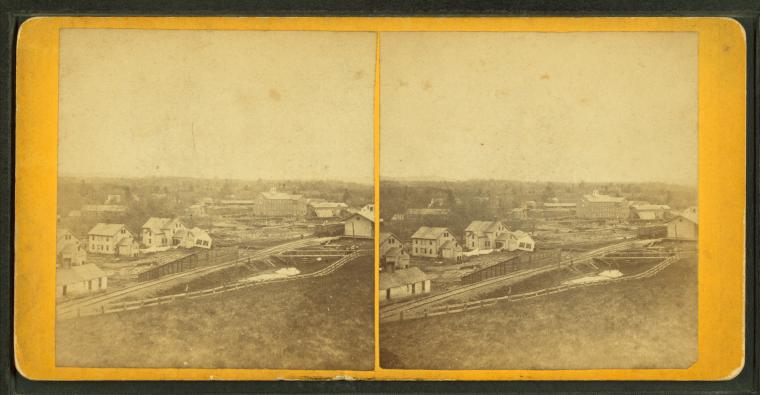
\includegraphics[width=10cm]{stereoscope}
	\centering
	\caption{Example of a stereoscopic image. \cite{leedsstereoscopic}}
	\label{fig:stereoscope1}
\end{figure}

There are a few more requirements for virtual reality platforms to consider in order to achieve an immersive experience and reduce motion sickness. A core fundamental feature of virtual reality is the ability to track head movements of the player in order for the game camera to adjust itself accordingly. IMU (inertial measurement unit) is a self-contained system in the headgear which measures linear and angular motion using multiple gyroscopes and accelerometers \cite{imu}. The device's IMU must be optimised and precise to provide accurate movement data as fast as possible since latency is another key factor.
\newline
\par
Latency as in most occasions is important to be reduced especially in virtual reality. Latency is the amount of time for a player action to be sent and registered to the game then for the game logic to compute this and display the consequence on the player's display. In the case of virtual reality, this would be the time for head movement to be registered and  the game to change the camera perspective to display in the virtual headgear. High latency would mean that the player will be seeing a delayed response of their actions which increases motion sickness as the brain is not seeing the expected response in a timely manner. This breaks the immersion and greatly increases chances of nauseea and motion sicknes.
\newline
\par
Another cause of possible motion sickness is the refresh rate of the headgear's displays. The refresh rate of a display is the amount of times a display updates it's image on the screen in a second. This also means that the refresh rate will determine how frames per sceond generated by a game will be displayed on the screen. A higher refresh rate display will allow games that can perform better by generating more frames per second seem smoother to the player's eyes. A low refresh rate would also introduce latency since the player's action cannot be displayed as quickly on the screen.
\newline
\par
Another key component of virtual reality that needs to be considered is the resolution of the display's screen. The resolution of a display is the amount of pixels that can be shown on the display so a higher resolution would mean a finer, more sharp image can be shown. This is important in virtual reality since the display is only millimeters away from the user's eyes so it would be easier for the user to distinguish individual pixels if the resolution is low.
\newline
\par
Virtual reality platforms have been released aiming to provide an immersive experience to consumers. There are many varieties currently available and they can be simply separated in to the two categories: mobile and desktop. Mobile experiences such as the Google Cardboard and Samsung's Gear VR target the audience which already own a compatible mobile device thus eliminating the cost of hardware found in higher end platforms. Through the use of the phone's built in gyroscope and accelerometer, crude head tracking can be achieved to emulate a virtual world.
\newline
\par
High end virtual reality platforms target enthusiasts and early adopters of cutting edge technology due to its premium price and high computer hardware requirements in order to run it. Currently there are two virtual reality headsets that are seen as the devices that give highest immersion and these are Facebook's Oculus Rift and HTC's Vive. These will be discussed later in this chapter.

\subsection{Mobile VR}
On the market right now there are two main mobile virtual reality hardware. There is the Samsung Gear VR and the Google Cardboard.

\subsubsection{Google Cardboard}
The Google Cardboard is the cheapest Virtual Reality headset out on the market right now, but it does come with the least features out of them. The cardboard viewer is a stereoscope made out of cardboard. It contains two 40mm focal lenses that are designed to give a distortion when looking through them, which is counter-acted by the distortion from the application\cite{cardboarddev}.
\newline
\par
To use the Google cardboard you would need to install the cardboard application on your compatible phone and then place your phone inside of the Google Cardboard. Once the phone is inside the Cardboard it uses the phone's IMU to track head movement. This does have limitations however as the Google Cardboard does not track displacement if the user was to walk in any direction.
\newline
\par
The Google Cardboard still uses the technology of stereoscopic images, as can be seen in \ref{fig:cardboard1}. Although it now does it with moving images, which creates a more immersive experience. \\

\begin{figure}[h]
	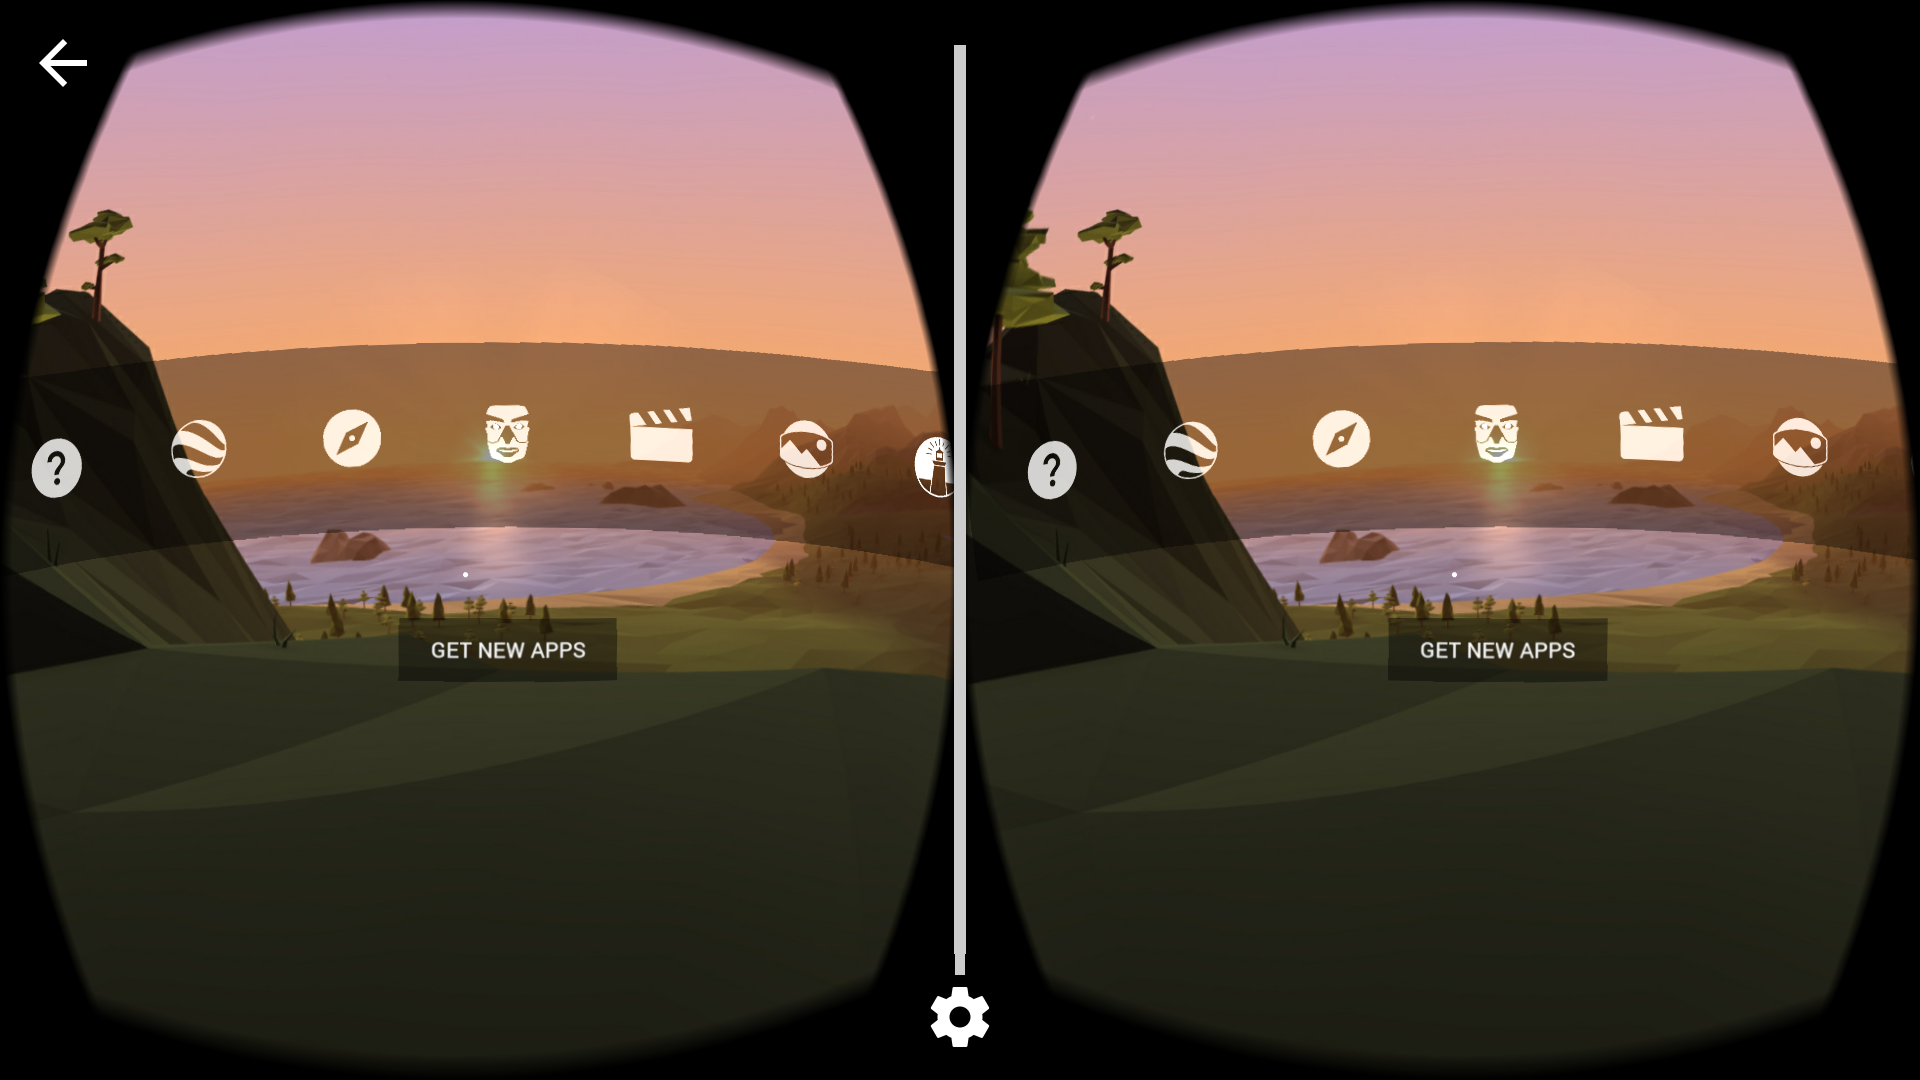
\includegraphics[width=\textwidth]{cardboardscreen}
	\centering
	\caption{Image showing the Cardboard demo application}
	\label{fig:cardboard1}
\end{figure}

The Google Cardboard was not chosen to the virtual reality device for this project as there are many drawbacks to it, and as such it does fully demonstrate all the features present in modern technology for virtual reality. The drawbacks to the Google Cardboard are:

\begin{itemize}
	\item No displacement tracking, making it less immersive than the other options
	\item Only one input method, a button on the cardboard which acts as a screen press.
\end{itemize}

\subsubsection{Samsung Gear VR}
The other mobile Virtual Reality headset on the market is the Samsung Gear VR. The Samsung Gear VR is slightly more expensive than the Google Cardboard, and as expected with the price increase, it comes with more features compared to the Google Cardboard.
\newline
\par
The Samsung Gear VR uses the same technology as the Google Cardboard in the sense that it uses stereoscopic imaging to create the illusion of depth. This is done in the same way for both VR devices, by inserting a compatible phone into the phone holder in the headset, and then showing the stereoscopic images on the phone screen. As seen in \ref{fig:gearscreen} the Samsung gear VR uses the same stereoscopic technology as the Cardboard uses, as seen in \ref{fig:cardboard1}.
\newline
\par
The Samsung Gear VR also uses an inertial measurement unit to detect head movement, similar to the Google Cardboard. The Samsung Gear VR uses an inertial measurement unit contained in the headset, rather than using the attached phone's inertial measurement unit. The inertial measurement unit contained in the headset is more accurate, has lower latency, and is better calibrated than standard phone inertial measurement units, as it uses the same I.M.U. as the Oculus Rift. This I.M.U. is more accurate as it has a higher sample rate than internal phone I.M.U.s and therefore gives it more values to use, so that it can more accurately detect erroneous values.

\begin{figure}[h]
	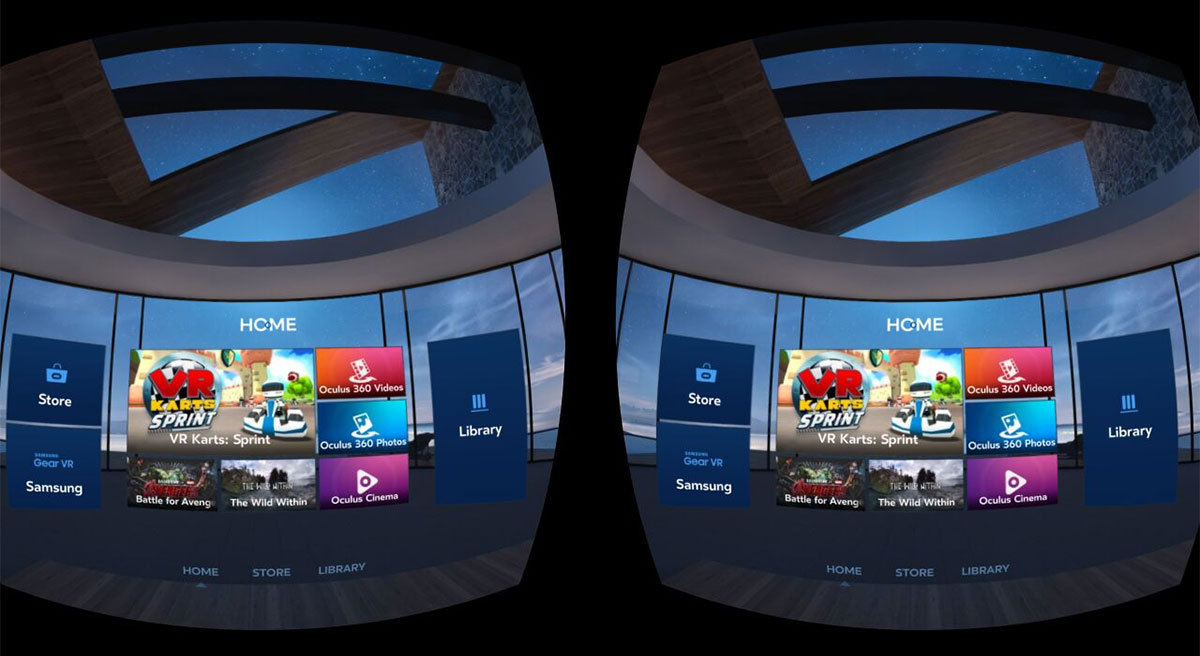
\includegraphics[width=\textwidth]{gearscreen}
	\centering
	\caption{Image showing the Samsung Gear VR menu \cite{gearmenu}}
	\label{fig:gearscreen}
\end{figure}

The Samsung Gear VR has a few extra features compared to the Google Cardboard, for example when a phone is placed inside the Galaxy Gear VR it needs to be connected by a micro-usb connection, which allows the headset to have more input methods to the phone, as well as giving access to the headset's I.M.U. The extra input methods that the Gear VR has access to are:\\

\begin{itemize}
	\item A home button, which works the same as the home button on Android phones.
	\item A back button, which works the same as the back button on Android phones.
	\item A touch pad, which works by swiping to move across menus, and tapping clicks the highlighted item in a menu.
\end{itemize}

\begin{figure}[h]
	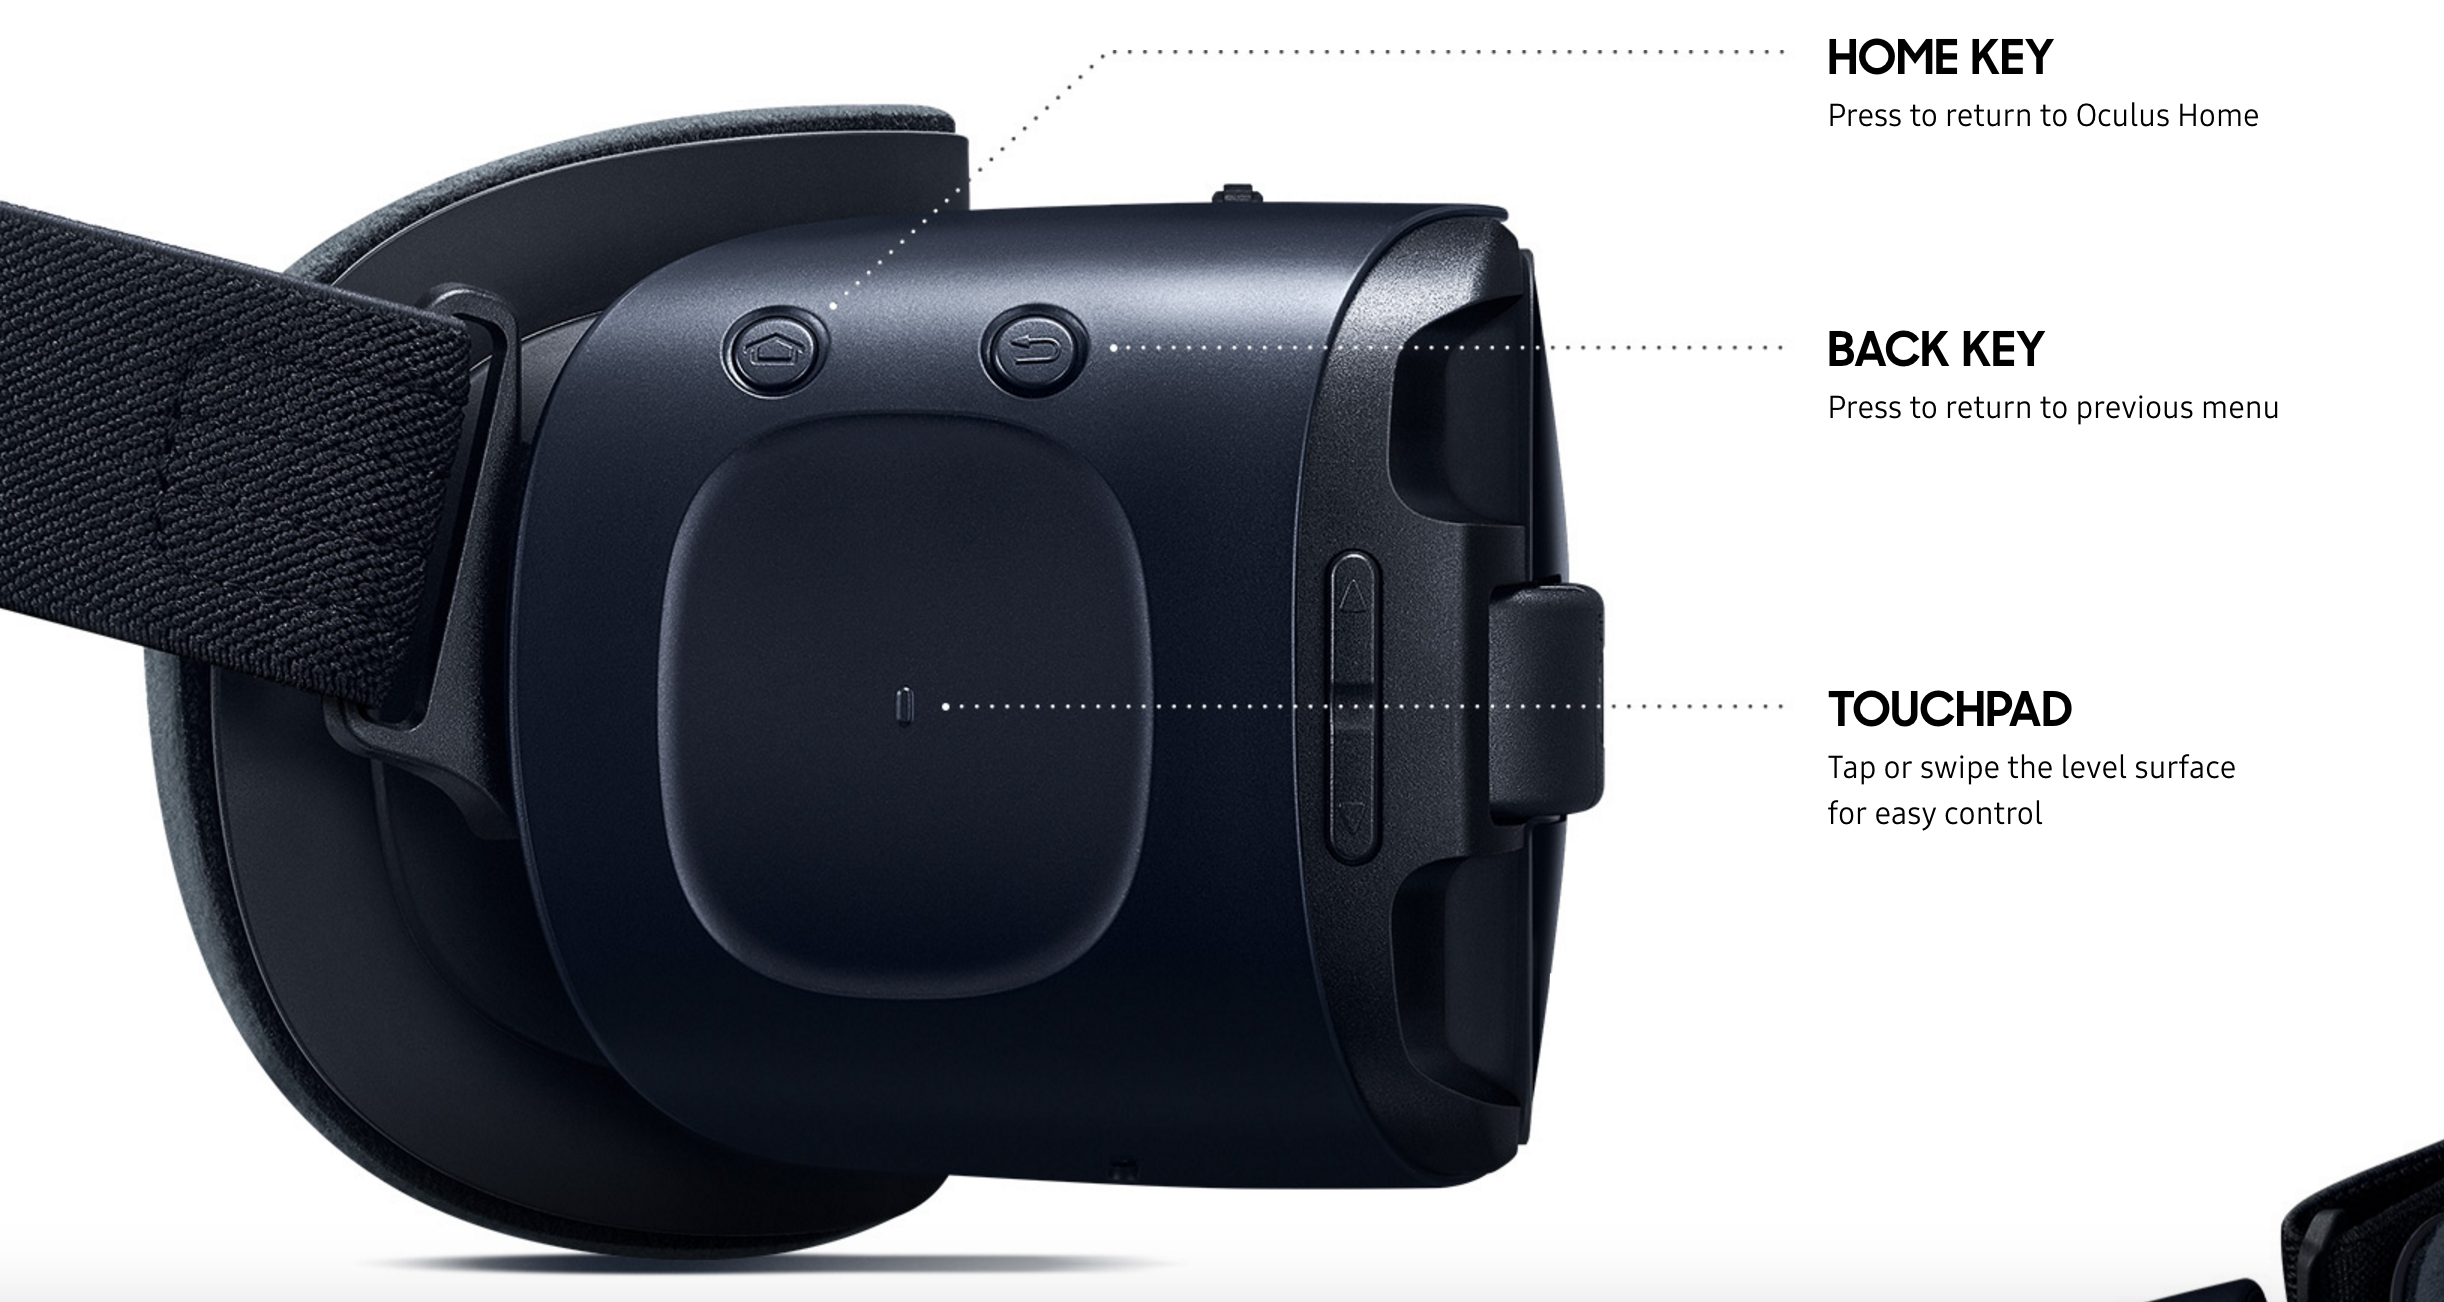
\includegraphics[width=\textwidth]{gearcontrols}
	\centering
	\caption{Image showing the hardware controls on the Samsung Gear VR \cite{gearbuttons}}
	\label{fig:gearcontrols}
\end{figure}

The Samsung Gear VR will not be used for this project as again it has several drawbacks, which are:

\begin{itemize}
	\item It only tracks rotational movement, not displacement, which makes it less immersive than the other options
	\item The Samsung Gear VR has very primitive control, which are only the buttons and touchpad on the side of the headset
\end{itemize}		


\subsection{Oculus Rift}
The Oculus Rift was the first of the two to be released and is inferior in terms of the level of immersion that can be achieved, as currently Oculus only supports interfacing with the virtual world through a third party traditional controller that simply uses buttons and joysticks. The Oculus Rift tracks by using the single camera to pick up infrared light that is emitted by points on the headset. These can be used to track the headset as they blink in a specific pattern, which the sensor knows, and it then uses that to determine the position the headset is in.

\subsection{HTC Vive}
The HTC Vive works using two base stations. These emit lasers in an alternating pattern, between vertical and horizontal. If these lasers hit a sensor on the headset or controllers, they emit a pulse. By tracking the timings of the laser sweeps and the emitted pulses, the tracking system can use trigonometry to find the position of the location of every sensor on the devices \cite{vivetechnology}. The HTC Vive has two settings, either a sitting or a standing mode. In the sitting mode, it works similar to the Oculus Rift, in that a gamepad is used to control the game, where as in the standing mode, it uses it's own controllers. The motion controllers which are tracked by the base stations provide a more immersive experience as it gives the player a more natural interaction with the virtual world. For example it allows the player to interact with objects in the game by using these controllers to pick things up by the player moving their hands to where the object is in game.
\clearpage

\subsection{Summary of VR Solutions}

\begin{table}[ht]
\centering
\begin{tabular}{|l|l|l|}
\hline
 & \textbf{Google Cardboad} & \textbf{Gear VR} \\ \hline
\textbf{Display} & Varies & OLED \\ \hline
\textbf{Resolution} & Varies & 2560 x 1440 \\ \hline
\textbf{Refresh Rate} & 60Hz & 60Hz \\ \hline
\textbf{Field of View} & Varies & 90-96 degrees\cite{fov} \\ \hline
\textbf{Tracking Area} & Static & Static \\ \hline
\textbf{Controller} & One button & Buttons and touchpad \\ \hline
\textbf{Sensors} & Accelerometer, gyroscope & Accelerometer, gyroscope, phone camera \\ \hline
\textbf{Requirements} & \begin{tabular}[c]{@{}l@{}}\cite{cardboardreq}Android phone:\\ versions 4.1 or higher\\ \\ iOS phone:\\ versions 8.0 or higher\end{tabular} & \begin{tabular}[c]{@{}l@{}}Gear VR compatible phone:\\ S6, Note 5, S7\end{tabular} \\ \hline
\end{tabular}
\caption{Comparisons table of mobile VR}
\label{mobiletable}
\end{table}

\begin{table}[h]
\centering
\begin{tabular}{|l|l|l|}
\hline
 & \textbf{Oculus Rift} & \textbf{HTC Vive} \\ \hline
\textbf{Display} & OLED & OLED \\ \hline
\textbf{Resolution} & 2160 x 1200 & 2160 x 1200 \\ \hline
\textbf{Refresh Rate} & 90Hz & 90Hz \\ \hline
\textbf{Field of View} & 110 degrees & 110 degrees \\ \hline
\textbf{Tracking Area} & 5 x 11 feet & 15 x 15 feet \\ \hline
\textbf{Controller} & Xbox One Controller & Vive controller, any PC compatible gamepad \\ \hline
\textbf{Sensors} & \begin{tabular}[c]{@{}l@{}}Accelerometer, gyroscope, magnetometer,\\ Constellation tracking camera.\end{tabular} & \begin{tabular}[c]{@{}l@{}}Accelerometer, gyroscope,\\ Lighthouse laser tracking system,\\ front-facing camera\end{tabular} \\ \hline
\textbf{Requirements} & \begin{tabular}[c]{@{}l@{}}NVIDIA GeForce GTX 960 / \\ AMD Radeon RX 470 or greater\\ \\ Intel Core i3-6100 / AMD FX4350 or greater\\ \\ 8GB+ RAM\\ \\ Compatible HDMI 1.3 video output\\ \\ 2x USB 3.0 ports\\ \\ Windows 7 SP1 or newer\end{tabular} & \begin{tabular}[c]{@{}l@{}}NVIDIA GeForce GTX 970 /\\ AMD Radeon RX 480 equivalent or greater\\ \\ Intel Core i5-4590 equivalent or greater\\ \\ 4GB+ of RAM\\ \\ Compatible HDMI 1.3 video output\\ \\ 1x USB 2.0 port\\ \\ Windows 7 SP1 or greater\end{tabular} \\ \hline
\end{tabular}
\caption{Comparisions table of desktop VR \cite{oculusvive}}
\label{desktoptable}
\end{table}

HTC Vive virtual reality hardware was chosen since overall it is the best amongst all the current VR solutions. The display hardware compared to the Oculus is the same, but the Vive offers room-scale experiences where the player can move around world. Also, motion controllers can be used to interact with the virtual world. These gives more immersion and the ability to develop experiences using these features.

% \section{Gaming}
% \lipsum[1-1] \cite{parikh1980adaptive}
\clearpage
\section{Development Environments}
To develop on the HTC Vive there are two options which are currently supported and these are the Unity engine and the Unreal 4 engine\cite{vivedev}. These game engines has native support for SteamVR which is the platform developed by Valve that powers the Vive. Both are free to be installed and just requires a simple registration to their respective websites.

\subsection{Unity}
Unity is a cross-platform game engine by Unity technologies and was initially released on June 2005\cite{unitywiki}. It was first announced only for OS X, but since then 20 more platforms have been added support \cite{unityhistory}. The game engine has support for development of both 2D and 3D games which is why Unity is popularly used in mobile games such as Temple Run. The cross-platform integration means that games can be quickly and easily ported onto other platforms such as Android, iOS and Windows. Unity currently supports the C\# programming language as well as Javascript for the development of games.\cite{unity3d}. Unity is a free to download and develop in, but games built using this engine will have the Unity watermark if the Pro version is not used which is a paid license.

\subsection{Unreal Engine}
Unreal Engine is the other game engine that supports development for the HTC Vive. This game engine is developed by Epic Games and was initially released on July 1998 \cite{unrealwiki}. It was primarily developed for first-person shooter games but then has found success in variouse other genres such as stealth and role-playing games. The first native scripting language used for game code and gameplay events in Unreal was called UnrealScript. This first appeared in 1998 and was used up until 2014 when Unreal Engine 4 was announced. Unreal Engine uses C++ on its current version and with this it means it is more portable and can be used by many developers. Like Unity, Unreal Engine is free for game development and only requires a payment of 5\% royalty on games and applications that are released\cite{whatisunreal}. This will not be a problem since the project will only produce a tech demo for non-commercial uses.
\newline
\par
With the current version of Unreal, Unreal 4, development for previous generation consoles are no longer supported. UE4 games can be released on PC, Mac, iOS, Android, Xbox One and Playstation 4\cite{unreal4nextgen}. This means that the engine can fully take advantage of bleeding edge technology and higher end graphics without having to worry about older technology. An example of the imporvement in graphics, UE4 can handle up to a million partices in a scene at one time whereas UE3 can only handle roughly a hundred.

\subsection{Unreal Engine: Choice for development}
Unity supports the C\# programming language for development whereas Unreal Engine uses C++ as its language of choice. Another aspect where it differs is Unity is mainly used to develop games for mobile devices such as 2D platformer games. Unreal Engine is mainly used for desktop, AAA games which makes it more suitable for virtual reality with games running on Unreal generally looking better.
\newline
\par
Unreal Engine includes many features built in such as particle effects simulation, terrain, lighting and shading \cite{unrealfeatures}. With SteamVR being natively supported, simple virtual reality features such as gesture recognition and teleportation movement mechanic can be easily implemented in to a game.
\newline
\par
For this project Unreal Engine will be used as the development environment. This is because the group is more comfortable with using C++ so development will be quicker with Unreal rather than trying to use a language with little familiarity. Syntax, grammar and structure of C++ will not be needed to be learnt and only special functions and members will be needed to be learnt and this can be easily done with the Unreal documentation. Along with Unreal's native VR support for headsets and motion controllers specifically for the Vive meant that learning to develop for the Vive will be easier.
\newline
\par
The Unreal Engine offers many features for people with little to no programming experience, these will not be used however, as they do not demonstrate any Computer Science expertise, one of the many features that will not be used is the drag and drop interface that is packaged in Unreal Engine to develop simple software quickly, along with the basic templates for various types of games. These are templates for popular genres, for example First Person Shooter and Sidescroller. For this project the group will implement their own features and backend for the genre that is picked, in order to demonstrate their ability to code for the HTC Vive. A select list of the features that Unreal Engine implements already are as follows:

\subsubsection{Unreal Engine 4 Features}
\begin{itemize}

	\item Particle Effects Simulation (Visual Effects)
	\item Procedural Foliage
	\item Landscaping/Terrain
	\item Lighting

	\begin{itemize}
		\item Directional
		\item Point
		\item Spot
		\item Sky
		\item Shadow Casting
	\end{itemize}

	\item Shading
	\item Post Process Effects

	\begin{itemize}
		\item Bloom
		\item Ambient Occlusion
		\item Colour Grading
		\item Depth of Field
		\item Lens Flares
	\end{itemize}

	\item Material Effects
	\item Fog Effects
	\item View Distance Culling
	\item Distance Dependent Level of Detail Models
	\item Physics Simulation
	\item Level Streaming (Ability load and unload map files into memory and toggle their visibility)
	\item Basic Templates

	\begin{itemize}
		\item First-Person
		\item Third Person
		\item Side Scroller
		\item Vehicle
	\end{itemize}

	\item Artificial Intelligence System
	\item Audio System
	\item DirectX 11 \& 12 Features

	\begin{itemize}
		\item Full-scene HDR reflections
		\item Per Scene Dynamic Lights
		\item Physically Based Shading
	\end{itemize}
\end{itemize}

Unreal Engine's full list of features can be found on their documentation site \cite{unrealfeaturelist}

\chapter{Requirements}
\label{chapter3}

In this section, requirements of the project are outlined. This is to easily define what problems and goals are to be solved by the project. Factors that are considered for the development of the project are mentioned in the feasibility assessment.

\section{Client Requirements}

The client has asked us to produce this technology demonstration in order to have a piece of software for the HTC Vive to demonstrate to students and has been developed by a University of Leeds student. The requirements that were given by the client were to appeal to the target audiences (who will be discussed in the next subsection), and to fully utilise the functionality of the HTC Vive in order to properly demonstrate its capabilities.

\subsection{Target Audience}
The demo would be targeted towards potential students looking to apply to the University of Leeds, as it will be shown to the students on open days in order to gain interest from them.
It would also have to appeal to people and companies in the gaming industry. As the more interest the School of Computing can gain from them, the more potential projects they may have for the school.
\newline
\par
With these target audiences in mind the demo should be technical to impress the gaming industry, while balancing it with being interesting for the potential students. This involves the implementation of features that are not trivial and not already built in the game engine.

\section{Feasibility Assessment}
\subsection{Feasibility}
To support the development of the project, a reserved space where the HTC Vive can be permanently set up for the duration of the project is required. This reserved space would ideally be a room that meets the space requirements stated above for room-scale experiences, so that all the capabilities of the Virtual Reality hardware can be used. A computer which meets the hardware requirements is also needed in order to run the HTC Vive software, This computer must be running Windows since HTC Vive currently only supports this operating system \cite{vivenolinux}. Also, a copy of Unreal Engine 4 game engine must be installed which is free to be downloaded. Unreal Engine 4 is chosen over Unity since the members of the group are more familiar with developing in C++ which Unreal Engine supports rather than C\# which Unity supports, although both of these game engines provide native support for virtual reality developments.
\newline
\par
A possible solution for meeting the hardware requirements is to use a personal machine. A laptop was available with the specifications below which just meets the requirements for the graphical power. Development can be done on our own personal Windows machines and can be tested with the Vive using the laptop in the reserved room. The Vive is not required for conducting simple tests, but it is needed for identifying issues such as scaling and user input with motion controllers.

\subsection{Technical Specifications}

\subsubsection{Hardware Requirements}
\begin{itemize}
	\item Graphics card: NVIDIA GeForce GTX 970 /Radeon R9 280 equivalent or greater
	\item Processor: Intel Core i5-4590 equivalent or greater
	\item RAM: 4GB+
	\item Video Ports: HDMI 1.4, DisplayPort 1.2 or newer 
	\item 1x USB 2.0 port
	\item Room-Scale Space: 2 meters by 1.5 meters
\end{itemize}

These requirements can be found on the official HTC Vive page on the Steam Store \cite{vivehardware}
\chapter{Project Management}
\label{chapter4}

This section describes how the project will be conducted throughout the project's development. Details on risks and problems that may arise as well as the contingency plan for them is outlined here.

\section{Methodology}
The methodology that will be used for this project is the Waterfall methodology. This methodology was picked as it is the most suitable for this project as agile works better with more experienced people working on the project as waterfall makes the planning and designing stages of the project more straight forward, which helps inexperienced people complete these stages. Some aspects of agile methodology will be used however, for example a weekly stand up meeting will be held, in order to discuss the plan for the following week. 
\newline
\par
Waterfall methodology was the chosen methodology for the development of the project due to the fact that we could completely design the demo using requirements agreed on at the start. Also with software deliverables being defined at the start it meant that planning and designing is more straight forward. This leads to progress being more easily measured since the fulle scope of the work is known in advance with tasks already set. The drawback with using Waterfall methodology is that it heavily requires on the effectiveness of the requirements. It must be made sure that the requirements is thorough so deveopment tasks can be made during the planning process because if requirements are changed throughout the development, then the schedule of tasks will be needed to be changed which will affect the progress of the project. Some aspects of agile methodology is used such as the client being heavily involved in the project due to the weekly meetings as this will give them many opportunities to see the work being delivered and to make decisions and changes throughout the development. These decisions must be small changes otherwise the project schedule will be heavily affected
\newline
\par
As part of the project schedule, there are two prototypes that are demonstrated to the supervisor. These prototypes shows significant development progress and features implemented. The first prototype shows a working demo with simple randomly generated graphs on flat ground as well as virtual reality features implemented. The virtual reality features will be limited to head and motion controller tracking in the game world, interaction with objects and teleportation navigation around the world. The second prototype will include terrain generation and Towers of Hanoi logic with water flow based on them. Having these prototype schedules makes sure that at certain points in the development there is a working product with features to show.
\newline
\par
The tasks outline in the project schedule in section 4.2 are evenly distributed for each member in the group. This is to maximise the amount of development that can be done so whilst someone is working on task, the other can work on a different task. This also helps with working on the project at the same time to avoid conflicts in code and development as each member is working on a different area.
\section{Project Schedule}
\begin{figure}[H]
	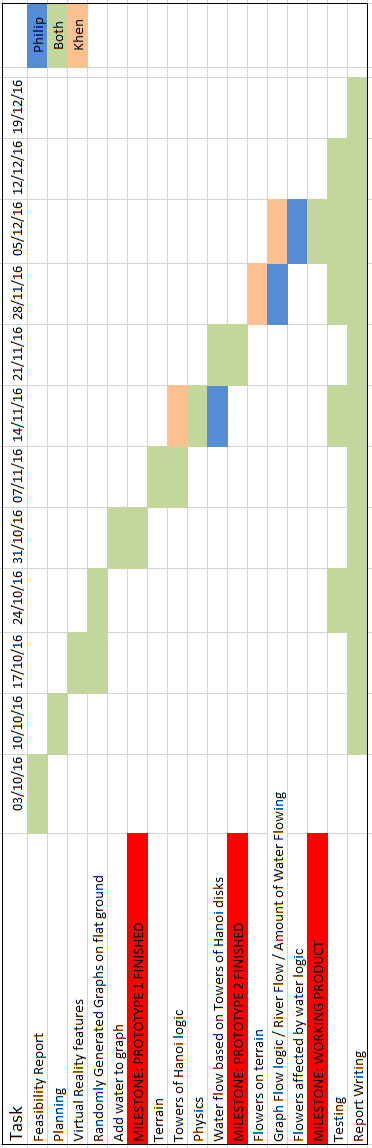
\includegraphics[height=23cm]{GanttChart}
	\centering
	\caption{Gantt Chart showing the work that will be done each week.}
	\label{fig:ganttChartPlan}
\end{figure}

\begin{tabular}{ |p{6cm}|p{3cm}| }
	\hline
	\textbf{Writing Milestone} & \textbf{Date For}
	\\\hline
	Layout Done & 14/11/2016
	\\\hline
	Chapter 1 - Introduction & 21/11/2016
	\\\hline
	Chapter 2 - Background & 28/11/2016
	\\\hline
	Chapter 3 - Requirements & 28/11/2016
	\\\hline
	Chapter 4 - Project Management & 05/12/2016
	\\\hline
	Chapter 5 - Planning and Design & 05/12/2016
	\\\hline
	Chapter 6 - Implementation & 12/12/2016
	\\\hline
	Chapter 7 - Testing and Evaluation & 12/12/2016
	\\\hline
	Chapter 8 - Conclusion & 12/12/2016
	\\\hline
	First Draft Complete & 12/12/2016
	\\\hline
	Report Finished & 23/12/2016
	\\\hline
\end{tabular}

\section{Version Control}
This project uses version control and a GitHub repository was created for this. Version control software will be used for the project in order to accurately document any and all changes that will be made to the code and the report write up. GitHub is the chosen version control service since it is the de facto standard for version control. Members are comfortable and familiar with using Git version control as opposed to others such as Mercurial. Version control is important for this project especially since it is a group project with multiple working on it at the same time. This makes it easier for collaboration through the use of merging. Also, with the use of commit history it can act as backups since they are created regularly just in case some new code broke the implementation so and older version can be easily loaded back up. The repository is also hosted remotely so it can be accessed using multiple machines and not just on one machine. This protects against losing files accidentally if it was stored locally. The GitHUb public repository is hosted using the following link: \url{https://github.com/kvcruzat/vivedemo}.

\section{Risk Assessment}
A risk involved with this project is the availability of the HTC Vive headset as well as its peripherals. Since the tech demo will be making use of the Vive as the virtual reality hardware, it is essential that a Vive is at hand to be used for testing the demo. The school currently owns 2 Vive packages and since the school is currently only using them for demoing purposes of off the shelf demos and not for development, a Vive should be available for the development in this project. If there is no access to a HTC Vive headset, a contingency plan has been made, which is outlined in \ref{subsec:conPlan}.
\newline
\par
Another risk that may occur is that the Vive has certain requirements for the space it needs to use for a room-scale experience. The Vive takes some time to set up since it has to recalibrate to the environment every time it is set up again. This means a dedicated room where the Vive's base stations can be left set up is ideal. If a big enough room is not available, Vive has an option to use a standing/seated experience instead. This will means that user movement cannot be tested and movement in the virtual world will have to be restricted to Vive’s teleportation mechanic. The user looking around the world will still be supported with this version.
\newline
\par
One other factor that needs to be taken in to consideration is the availability of computer hardware that is powerful enough to run and develop on the HTC Vive. Since the HTC Vive has high minimum requirements to run it, finding a computer that is sufficient and can be used when needed can become an issue.

\subsection*{Contingency Plan}\label{subsec:conPlan}
In the case that there is no access to a Vive headset for this project, due to the risks mentioned before, a contingency plan has been made. The plan would be to make a desktop application using the same premise, rather than being able to use the Vive for the game. This desktop application would have the same features as the Vive version, although without the VR features, i.e. looking around using the headset and interacting with objects using the controllers.
\newline
\par
The plan for dealing with if there is no room available is that a seated experience could be developed without need a room set-up. This would just involve setting up one camera above the computer and it would only track head movement. A standard game controller would have to be used for this set-up.
\newline
\par
For the risk that there is no high-end computer available, a high-end laptop that can run the software has already been acquired and will be used if there is no other computer available. The laptop is personally owned so there is no problem in accessibility.
\chapter{Planning and Design}
\label{chapter5}

\section{Game Design Process}
	The game design process started by using the HTC Vive to research what kind of games were already on the market for the HTC Vive. The games that were SteamVR Demo\cite{steamvr}, The Lab\cite{thelab}, Space Pirate Trainer\cite{spacepiratetrainer}, and Elite Dangerous\cite{elitedangerous}. This research was done in order to give a feel for the HTC Vive and it's capabilities, this would give a clearer understanding to which kind of games are more suited to the Virtual Reality platform.\\
The next step in the game design process was to brainstorm ideas of what kind of game would be made for the project. The ideas would be split into four categories, these four categories are the theme of the game, the features of the game, the genre of the game, and the benefits of the game.\\
% Needs picture of whiteboard or formatted table %
The brainstorm was then categorised in a separate table, combining the ideas that have relevance together, this table can be seen in \ref{}.
%Insert neat table here%
Then using the updated table of ideas, the ideas were narrowed down until one that could feasibly done was chosen out of all the ideas on the white-board. This idea was to combine the Towers of Hanoi and Graph Flow in a puzzle game. These two ideas were combined in order to make a technology demonstration that is very specific to the School of Computing in the University of Leeds, as these are both topics of study during the Computer Science course in the university of Leeds.\\
A goal for the game then had to be designed. The goal of the game was decided to be having the right amount of flow run down to set nodes, where flowers would be. If these flowers have too much water flow they would look dead, and if they had too little water flow they would also look dead. They would only look alive if the water flow was the correct amount. The game is won when all the flowers are "alive" at the same time.\\
	This idea would implement many non-trivial features in the Unreal Engine, such as:
	\begin{itemize}
		\item Randomly generating a graph
		\item Generating a terrain based on the graph
		\item Towers of Hanoi logic for flow control
		\item Having plants being affected by the water flow
		\item Changing the appearance of the water, based on the flow of that edge of the graph
	\end{itemize}


\section{Virtual Reality Features}
The Virtual reality Features that will be used are:
\begin{itemize}
	\item Using the Head Mounted Display in order to look around the virtual world.
	\item Using the controllers to pick up the Towers of Hanoi disks, and place them down.
	\item Using the controllers to select a teleport location to move.
\end{itemize}

\section{Graph Flow}
Graph Flow will be used in this technical demonstration as the main objective of the game. The objective of the game will be to get the flow to match the goal flow. This will be done by blocking off certain rivers to redirect flow from one river into another. The goal flow will be calculated in development, and each level that is created will also have a goal state completed.

\section{Towers of Hanoi}
Towers of Hanoi will be used in the demo to block off the graph flow from nodes to other nodes. This will be done by having rods in the river at each split in the graph. These will be placed at the output of each split in the river. The Towers of Hanoi disks will then be placed on top of these rods if the flow needs to be blocked. The Towers of Hanoi disks will only be allowed to be placed in the opposite order compared to the way the normally are. This would mean that a larger disk can only be placed on top of a smaller disk. This order had to be inverted to the standard as rivers are narrower at the bottom, compared to the top of the river ditch. 

\section{Plant Survival}
The Plant Survival will be used as a measure for the player to determine how close he is to solving the puzzle. This will be the indicator to the player if the flow at that node matches the pre-determined flow for the level
\chapter{Implementation}
\label{chapter6}

\section{Development Environment}
The development of this project was done in various environments, as there was many different aspects to this project.

\subsection{Vive Hardware}
For this project, the Vive Hardware was set up in a dedicated room (The Virtual Reality Lab in the School of Computing). This allowed development to be done on the HTC Vive without having to set up the sensors and calibrate the hardware every time that development had to be done, which maximised the amount of development time that was available.

\begin{figure}[H]
	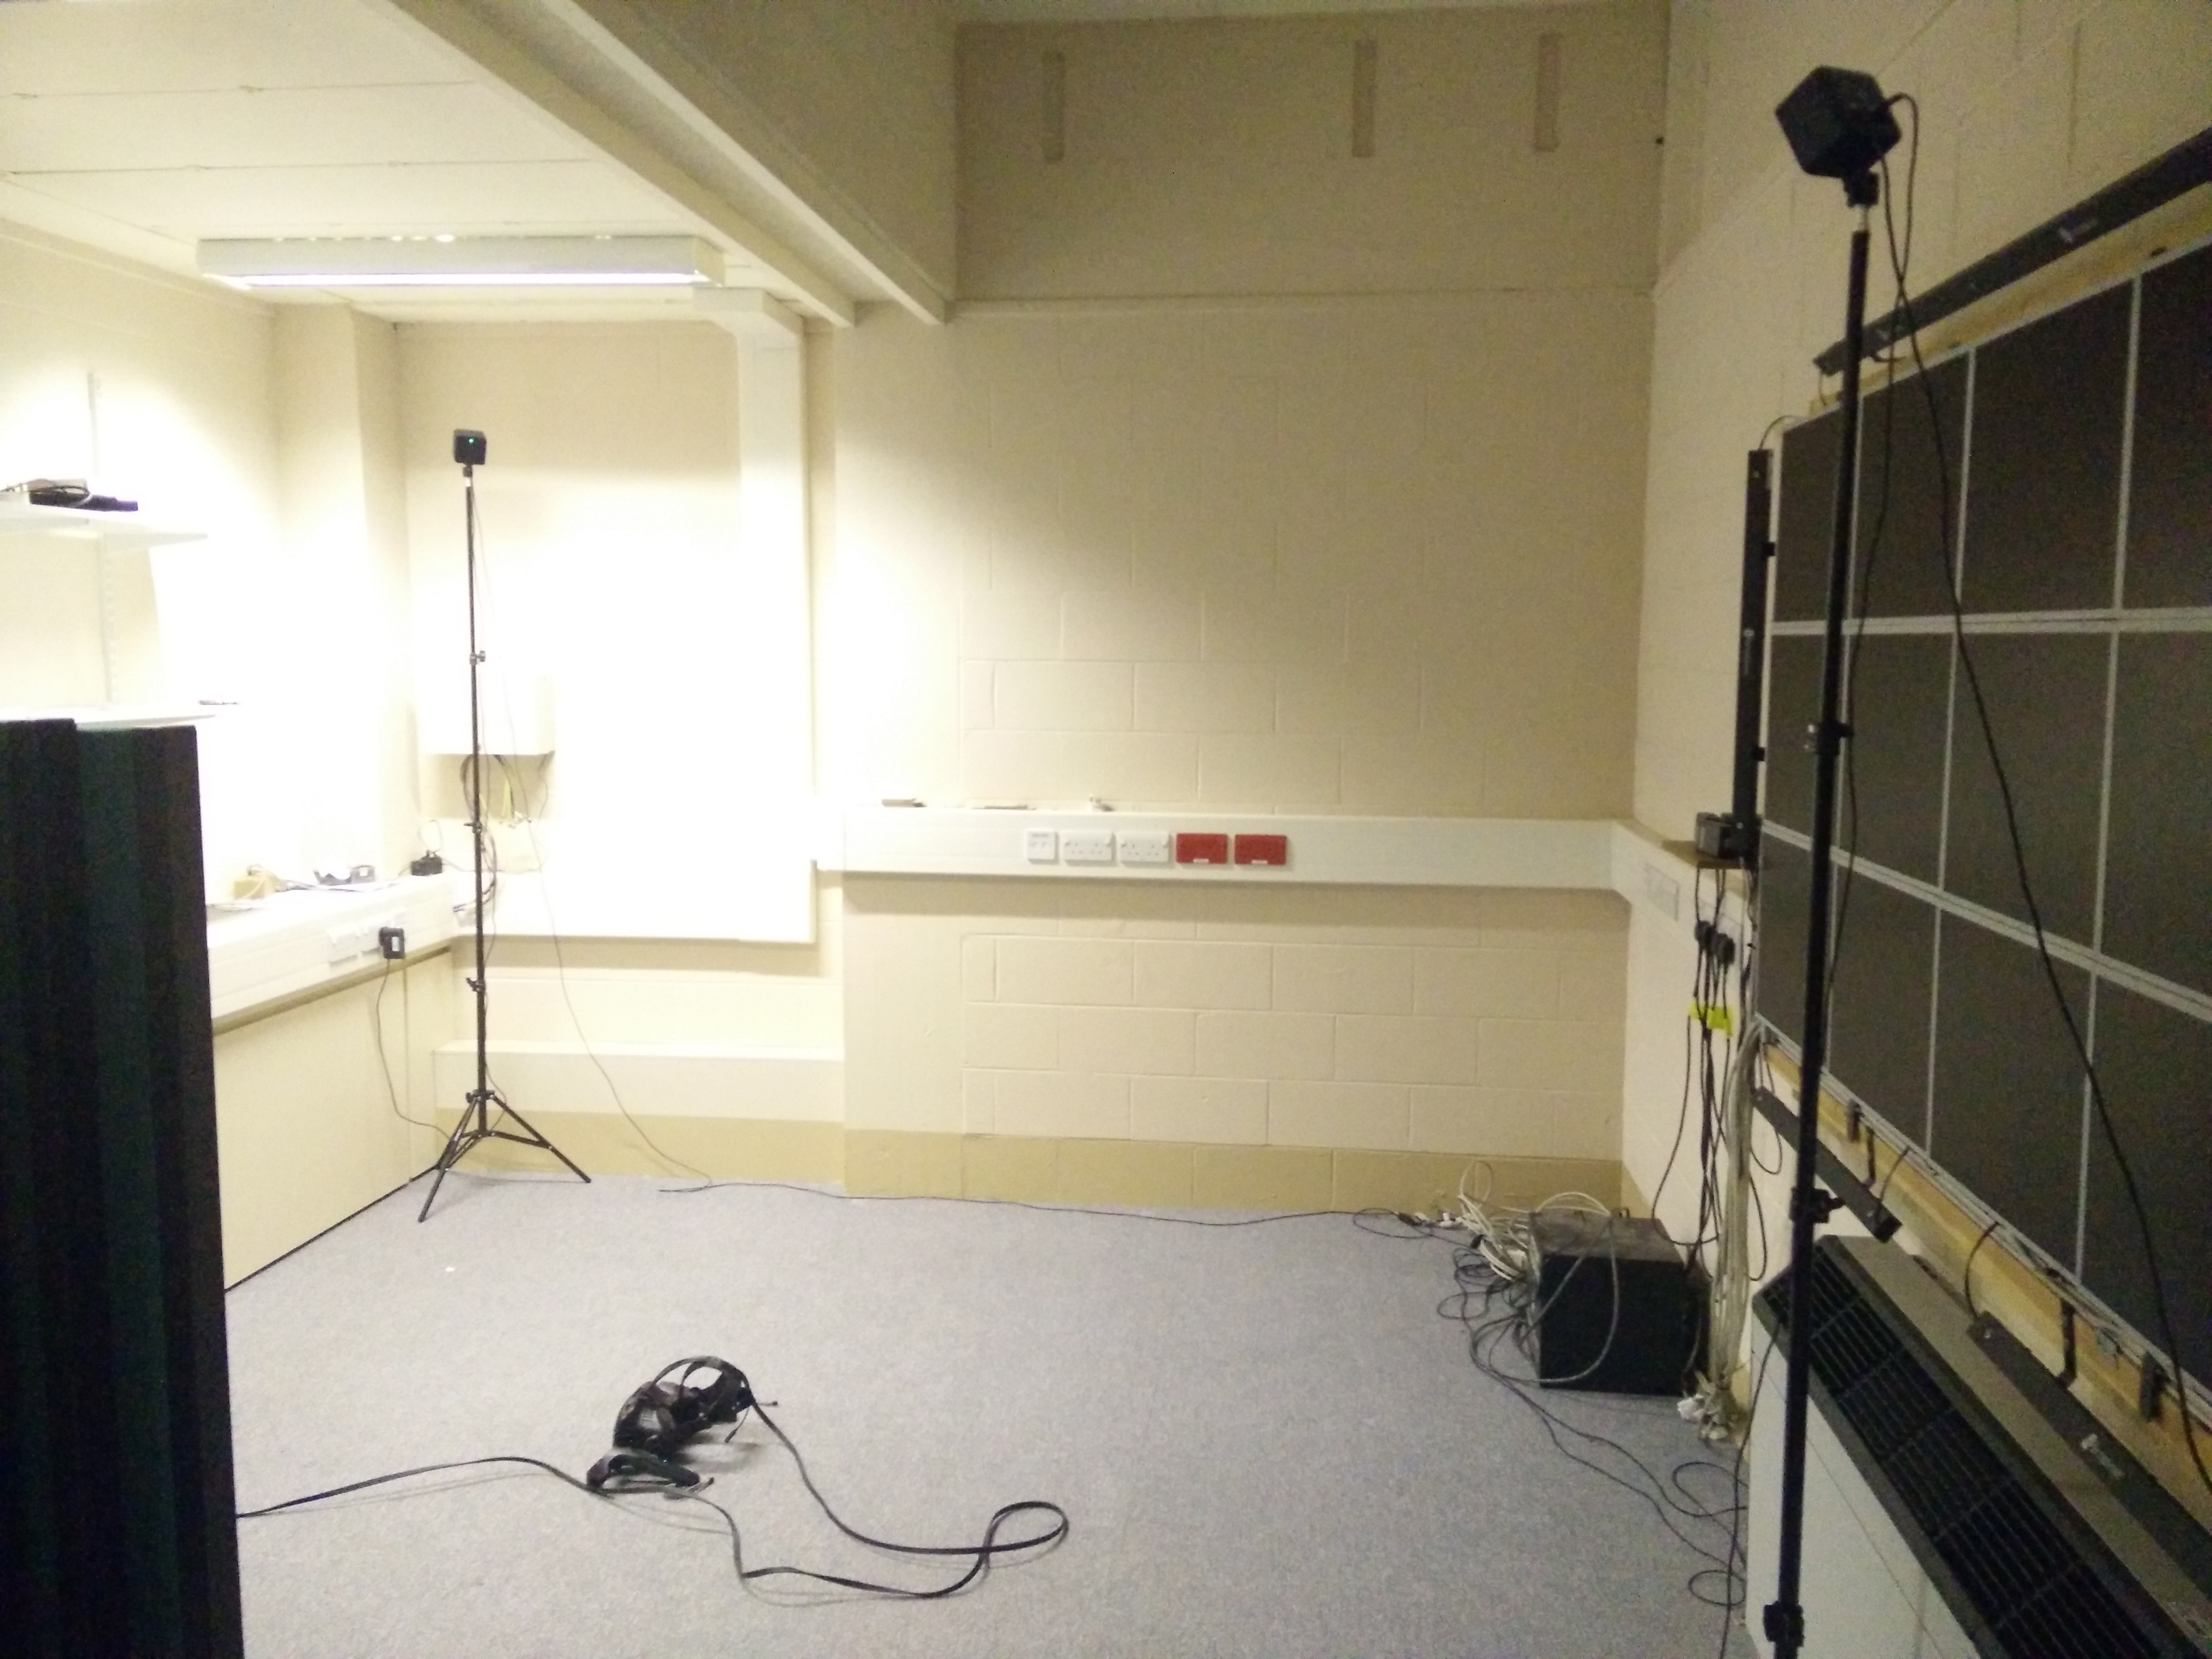
\includegraphics[width=\textwidth]{VRRoom}
	\centering
	\caption{Room used for testing the application}
	\label{fig:VRRoom}
\end{figure}

This room was chosen as it was unused and met the space requirements for the HTC Vive. Approximate room space available resulted in 2.9m x 2.9m which is more than sufficient.

\subsection{Game Engine}
 The chosen game engine used for development as stated in chapter 2 is Unreal Engine. The latest version as of the time of development was used which was Unreal Engine 4.13.2. This decision was made to make sure bugs that may have appeared in previous versions were fixed and also for new features to be taken advantage. Since virtual reality is bleeding edge technology, new features and ways to use VR in development are being implemented rapidly. When development started an older version was being used and new updates were being rolled out, the group decided to update the development environment when a new update was released. It was made sure that everyone in the group was using the same version of Unreal to avoid backward compatibility issues.

\subsection{Visual Studio}
When developing in Unreal Engine, the editor used was Visual Studio. Unreal Engine was designed to integrate smoothly with Visual Studio so code changes can be built in Visual Studio and then can be quickly seen in the Unreal Editor. It also provides a debugging tool to help solve code problems and bugs due to the fact that it has knowledge of the Unreal API. Visual Studio's Intellisense feature has the ability to list members, methods and parameter information when coding. This helped with learning the API, making it easier to detect syntax errors before compiling. The version used was Visual Studio 2015 since Unreal Engine versions 4.10 or later must use this version and not the older 2013 version.

\subsection{Windows}
The operating system used was Windows 10 since the SteamVR software that powers the HTC Vive is only compatible on Windows operating system as of the time of development. Windows 10 was the version that was the latest version and the personal systems the group members owned that were used to develop was already running Windows 10 which made it more convenient to use.

\subsection{Out of Engine Development}
The out of engine development was done in C++, using Sublime Text as an editor, this decision was made out of familiarity with the software. Some C++11 functions and types were used in the development of the graphs, rivers and terrain. The generation for these was done without the use of the Unreal Engine as it outputs files that are then read in with the Unreal code to help generate the game terrain, objects and logic.

\section{Random Generation of Graphs, Rivers and Terrain}

%Divide into sub sections as big topic
\subsection{Graph Generation}\label{subsec:graphGen}
	This section will highlight the main points in the algorithm developed to generate a graph that would be usable by the technology demonstration.

\subsubsection{Start Point Generation}
	The method to generate the starting graph was to start with an empty matrix of nodes, of a size determined by a global variable. These nodes are then all connected using 8-connectedness. This means each node is connected to the eight nodes around it. This makes a graph that looks similar to \ref{fig:triangulation7}.

\begin{figure}[H]
	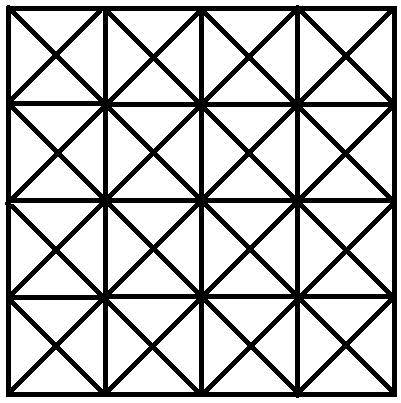
\includegraphics[width=10cm]{triangulation7}
	\centering
	\caption{Image showing an example of the new method of connection the nodes, where the starting matrix is 5 x 5.}
	\label{fig:triangulation7}
\end{figure}

	This produces a connected graph which contains several edges for the connections between nodes to use.\\

\subsubsection{Connections and Weight Matrix}
	The starting set of nodes is found by first selecting the top-left and the bottom-right point as starting nodes, and then randomly selecting others until the amount of nodes selected is the same as the variable stating how many nodes should be selected.
	\newline
	\par
	The weight matrix was made using Manhattan distance between the two connected points as the heuristic. The Manhattan distance is the x distance between the two points plus the distance in the y direction. The Manhattan distance was calculated using the following formula:\\

	$$Manhattan = (point1.x - point2.x) + (point1.y - point2.y)$$
	
	The Manhattan distance then has to be checked to see whether it is positive or not. If it is positive the result is put in element of the matrix representing the first point to the second point, if the result is negative the result is instead placed in the element representing the second point to the first point. This is repeated for each connection in the connection matrix produced before.

\subsubsection{Generating Rivers}
	To generate the rivers the algorithm must first decide which nodes should have rivers running between them. It does this by first finding the distance from the top-left to each of the selected nodes. It then loops through the selected nodes and tries to find two connections where the flow is going downwards. It makes sure the flow is going towards the bottom-right by checking the distances, and if the distance is larger on the node it is trying to connect to, then the river is flowing to the bottom-right. There is a for-loop that will loop through each node, in the order of smallest distance from top-left to largest distance from top-left, looping in this order gives the benefit that the closest nodes to the current will always be selected to connect.\\

	%findConnections code snippet%

	The next step is using Dijkstra's algorithm to find the shortest path between each pair of connected nodes.\\

	%Code snippet for dijkstra's?%

	Using the shortest paths generated by Dijkstra's, a new connection matrix is made. This connection matrix is made by looping through each path made by Dijkstra's algorithm and looking at each pair of nodes. These pairs would be the consecutive nodes in each path. After this connection matrix has been made it is time to map out the graph, so that it can be transferred to the terrain. Mapping out the graph is done by having a matrix of the same size as the terrain will be, this matrix is initialised to have all ones, as the lines will be modify the elements to be 0, as they will be ditches. Then by looping through the connection matrix made before, the connections will be drawn onto the matrix. The connections are drawn onto the matrix by first checking if the element in the connection matrix is 0 or 1, 1 being that there is a connection between the two nodes. If there is a connection then the line between these two points should be drawn onto the height map matrix. This line is calculated by using a modified Bresenham's Line Algorithm, the algorithm is modified so that it can be used in all eight octants of a graph, rather than just the octant that the line goes down and to the right. This modified algorithm is explained in more detail in the section below.

	%Code snippet for drawing lines?%

	The coordinates are then updated so that the coordinates align with the size of the grid, instead of just being consecutive numbers. The coordinate updating is done by first getting the scale factor for the points. The scale factor is the size of terrain divide by the size of the starting matrix, rounded down. The coordinates are then looped over and each x and y coordinate are multiplied by the same scale factor, as the terrain is always square. The last point (the bottom-left point) is then set separately, as it should be set to the bottom-left of the terrain. \\

	%update coordinates code snippet%

	After the coordinates have been updated it is time to generate the connections matrix, this is done by looping over the shortest paths and setting each element in the matrix, that represents the consecutive pairs in the shortest path, to be connected. While the generation code is doing this, it also is determining which nodes should be the "new" nodes. These "new" nodes are where the intersections are in the graph, as the previous nodes are not always guaranteed to be at an intersection. These "new" nodes are used later on in the program in order to decide where to place the rods in the game.
	\newline
	\par
	The program determines which nodes by checking which nodes have been used two times or more. It does this during the for loop when it generates the connection matrix, whenever a element in the connection matrix is set to be connected, then it loops over the array that stores all the connections that have already been used, and checks if the first point of the used connection is the same as the first point in the connection that has just been stored in the connection matrix, it also checks to make sure the second points are different. If the two first points are the same and the two second points are different, then an intersection has been found. The algorithm will then check the array of already found "new" nodes, to make sure that the node doesn't already exist in the array. If it does not exist in the array, it is added to the array, the used connection is then added the array storing all the used connections.\\

	%printGraph snippet%

	After the previous step comes removing edges from the graph that either act as either a sink for the graph, i.e. there are no connections after it, or it acts as a source for the graph, i.e. there are no connections leading to it, as the graph should only have one source, the top-left, and one sink, the bottom-right. The first step in this algorithm is to determine how many times each node has been used as a starting node (being used as the first point in a connection), and how many times it's been used as an end node (being used as the last point in a connection). This is done by looping over the used connections array from the previous step, from each element of this array the start node and end node is extracted. The corresponding nodes then have their respective values incremented in an array for both start nodes and end nodes.
	\newline
	\par
	One of the two cases that are being removed is when a node is not used as an end node, but it is used a start node one or more times. In this case the node would be a source node. This node is then placed in an array of nodes that are removed the graph, and should not be included in it. Now the algorithm needs to look at the nodes that the removed node was connected too, and see if they should be removed. This is done by implementing a stack. The nodes that are connected to the removed node are placed in the stack. This is implemented by having two while loops. One of the while loops is checking to see if the stack is empty, the other is checking if the end of the path has been reached, this being the inner while loop. The end is found when the algorithm can not remove any more nodes from that path. Inside the while loops there is a for loop, looping over the used connections array. For each iteration of this for loop, the start and end node are extracted. The start node is then compared against the node that is being looked at by the algorithm, if they are the same it then checks if there is more than one end node and if the node does not exist in the removed array. If these are both true then the algorithm adds the node to the removed array. The algorithm then needs to find the nodes that are connected to the node that was just removed. The number of connections is found by looping through the connections array and extracting the start node of each element, and incrementing a counter every time the start node matches the removed node. If only one connection is found then the inner while loop carries on, but the current node is now the second point in the connection that was being looked at when the node was removed. If there is more than one connection then every connection found after the first one will have the end node extracted and added to the stack. The end of the inner while loop can also be found if it completes one full cycle of the used connections array without finding any node to remove.
	\newline
	\par
	Once the end of the path has been found, the algorithm will check the size of the stack, if there is nothing inside of the stack, the algorithm will stop. If there is something inside of the stack, the algorithm will use the top value to start its search for nodes to remove, and then remove it from the stack.
	\newline
	\par
	To find the sink nodes the algorithm uses the same method, but instead of using the first node in the connections, it will use the last node of the connections, and whenever the last node was used in this previous part, it will used the first node.
	\newline
	\par
	
	%printGraph snippet%

	The next step of the algorithm is generating the height map for the graph. This is done similarly to the previous method, but with a few notable differences. These differences are in regards to output. In this version of the code, the algorithm needs to output where the rivers and rods are located on the terrain. These are found by first checking if the first node of the connection is a selected node, if it is the line drawing will also record the place that the rod should go. At the first iteration of the line draw algorithm, it records the x and y position of the river for the first side of the river. The x and y coordinates depend on how steep the line is. If the line is 45 degrees or more then the x coordinate is the line's x coordinate plus the river width for one side and minus the river width for the other side. The y coordinate remains the same. If the line is less than 45 degree, then it is the y coordinate which changes with the river width. The same is done for the last iteration of the line draw algorithm. The name of the river is also stored in an array, the name is simply the two nodes that it is connected too. If the line came from a selected node, then a rod needs to be placed. The location of the rod is the same as the line on a set iteration.
	\newline
	\par

	%code snippet%

	After the lines have been drawn, it is time to expand them on the height map, this has to be done so that the connections look more like rivers in the demo. This widening is done by taking a copy of the height map and using the copy to modify the original. The copy of the height map is then looped through, checking each element of the height map. If the original height map is equal to zero, meaning that a line has been drawn in the element, then the algorithm will try to change the value of the pixels in set distance away from this pixel in both the x and y direction, this distance is set as a global variable. The algorithm changes the values of the elements of the copy height map within the range depending on how far away the elements are. Within a third of the distance away the value is set to zero, within two-thirds of the distance then the value is set to $0.33$ and just within the distance it sets the element to $0.66$, this is done as in the game the Towers of Hanoi discs will need to fit inside the rivers, and have their own platform to rest against, and as there are three discs, the distance is split into thirds. The original height map is then replaced by the copy of the height map.
	\newline

	%Code snippet for making ditches

	\par

	The program then needs to recalculate the shortest paths between the nodes, as it needs to output connections between the "new" nodes. This is done using a greedy algorithm, this algorithm will be given a starting river, then in a while loop it will first check if the end node of the river is one of the other "new" nodes, or if the end node is the bottom-right node. If either of these are true, then it will break the while loop. If they are both false, then the greedy algorithm will find the first river that connects to the end node, set the new river as the current river and then the while loop will start again, and it will carry on until it reaches an end node. The algorithm will then return the path it found to the next node.
	\newline
	\par

	%greedy snippet%

	Once all the new shortest paths have been found, these will be output to a file that will be used by the game, so that the game knows the route that the rivers take.\\
	The next step of the program is determining which directions the rivers are flowing into a node, and flowing out of a node. This directions must be found as the game will use this information in order to know where not to place flowers on the terrain. This is done by looping through the new paths and extracting the start and end node from th paths. The algorithm will then search through the array and see if either the start node or the end node is one of the selected nodes. If the node is one of the new selected nodes, then it will check which direction the river came from by comparing the start and end node of the river to each other. As each direction has a distinct amount of difference between them, the direction it is going can be determined. These directions are then output to a file for the game to read in.\\

	%directions snippet%

	At the end of this program the output will look like \ref{fig:triangulation8}

\begin{figure}[H]
	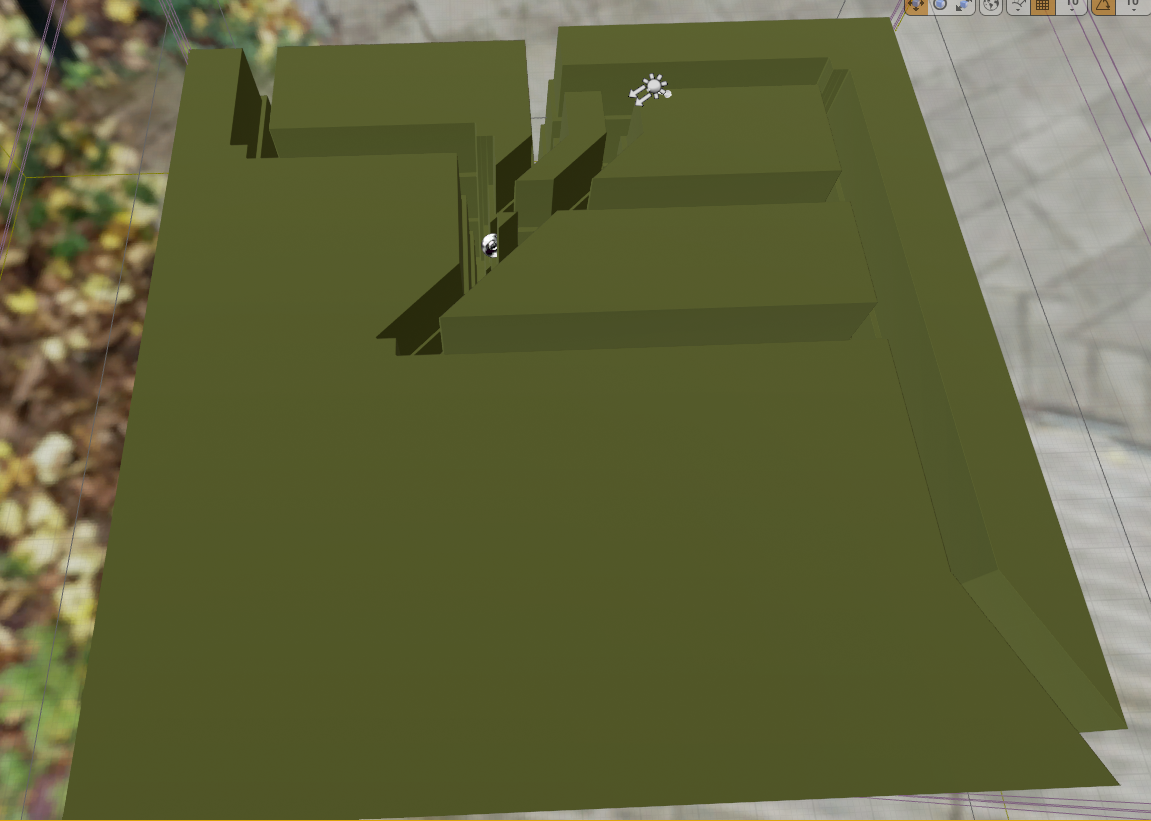
\includegraphics[width=\textwidth]{triangulation8}
	\centering
	\caption{Image showing the output without any randomly generated terrain.}
	\label{fig:triangulation8}
\end{figure}

\subsubsection{Bresenham's Line Algorithm}
	\par
	Bresenham's Line Algorithm is a rasterisation algorithm, it works using error checking for the y coordinate. The original Bresenham's Line algorithm works by finding the absolute value of the gradient, then it loops through each point in the x direction of the line segment. At each iteration through the line it adds the gradient to an error value, when this error value ticks over the value $1$, it will increment the y value of the coordinate for the rest of the iterations. At each iteration of the algorithm, it will plot the point of the current x and y coordinate onto the height map.\\
	The modified Bresenham's Line Algorithm that is used in this project does the same thing, but it lets the algorithm work for lines that are not sloping down and to the right. The modified version does this by first checking the gradient and if the gradient is over $1$ or under $-1$, then the algorithm will swap the x for the y values and the y values for the x values, so that the gradient is less than $1$ and greater than $-1$. The algorithm will then check if the line is sloping to the left or right, the check is comparing the x value of the first point to the x value of the second point and seeing which is bigger. If the line is sloping to the left, the algorithm will swap the points, so that the first point becomes the second point, and the second point becomes the first point. The last step the algorithm takes to ensure that it will work, is that it will check whether the line is sloping upwards, or downwards. If the line is sloping upwards, it will set the change in y to be $-1$, so that it subtracts from the y value, rather than adding it.

	%Code snippet for line drawing%

\subsection{Graph Generation Original Method}\label{subsec:GGOM}
This section will outline some of the previous iterations of the algorithm used to generate graphs, and why these algorithms did not succeed.
\subsubsection{Point Insertion}
\par
	The original idea to do graph generation was to start with a square, using each corner as a node. These nodes would then be connected as shown in \ref{fig:triangulation1}.\\

\begin{figure}[H]
	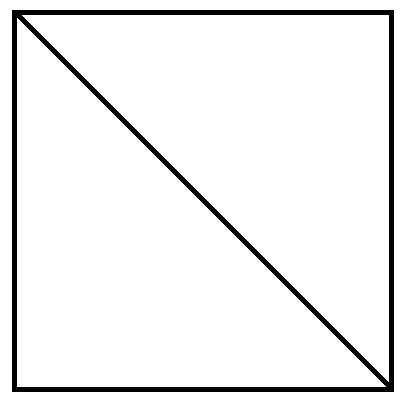
\includegraphics[width=10cm]{triangulation1}
	\centering
	\caption{Original Connections}
	\label{fig:triangulation1}
\end{figure}

	Points would then be inserted into this square, using a random x and y value.  The triangle that this node is in would then be found using the cross product. This was done by checking the cross product of the point and the triangle, for each triangle that is in the graph. The point would then be connected to the corners of this triangle.\\

\begin{figure}[H]
	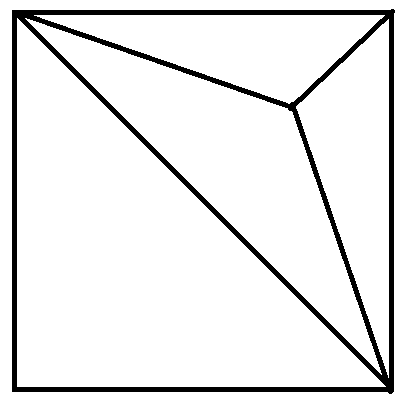
\includegraphics[width=10cm]{triangulation2}
	\centering
	\caption{Example of running the point insertion algorithm for one iteration.}
	\label{fig:triangulation2}
\end{figure}

\begin{figure}[h]
	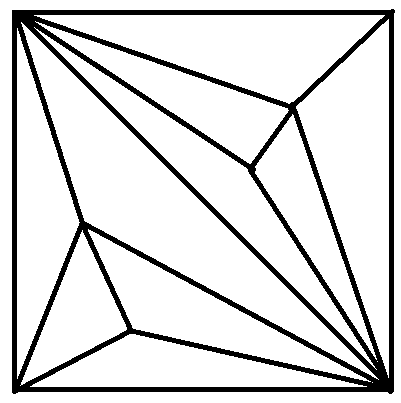
\includegraphics[width=10cm]{triangulation3}
	\centering
	\caption{Example of running the point insertion algorithm for four iterations}
	\label{fig:triangulation3}
\end{figure}

	This approach guaranteed a connected graph to begin with. This approach did not work however as if a node on the bottom-left side of the graph needed to be connected to a node on the top-right side of the graph, the the connection would have to be made through either the top-left node or the bottom-right node, as there was no other way to pass through to the other side of the graph. The approach was then modified slightly to start with an extra node node in the middle of the square, allowing another way to pass through the other side of the graph, this is seen in \ref{fig:triangulation4}.

\begin{figure}[H]
	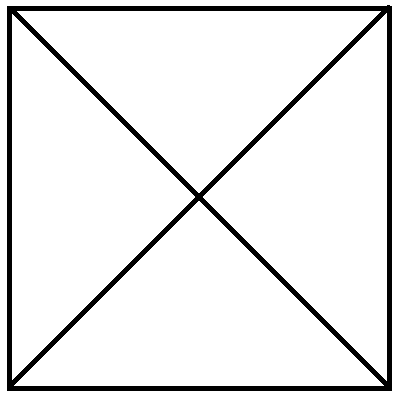
\includegraphics[width=10cm]{triangulation4}
	\centering
	\caption{Image showing the second method's starting connections}
	\label{fig:triangulation4}
\end{figure}
	
	This approach also did not work, as the addition of the extra node did not provide enough of relief for the connections between the two sides of the graph, and the connections would occasionally still go through the top-left or bottom-right node.
The next approach was adding several nodes along the diagonal and connecting them to the corners, similarly to how the middle node was added. The third approach can be seen in \ref{fig:triangulation5}.

\begin{figure}[H]
	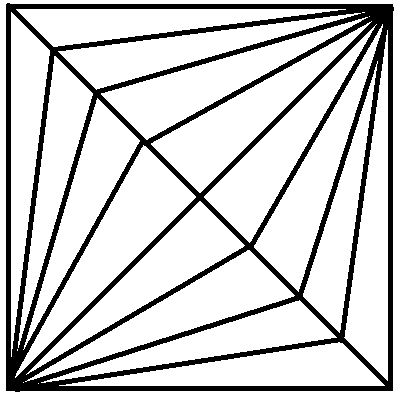
\includegraphics[width=10cm]{triangulation5}
	\centering
	\caption{Image showing the third method's starting connections}
	\label{fig:triangulation5}
\end{figure}
	
	This approach also did not work as when the shortest paths between nodes were found, the paths tended to favour the path from the top-left to the top-right. This would make the graph just be a straight line, with a few edges going to the nodes that were used in the river graph, an example of this can be seen in \ref{fig:triangulation6}.

\begin{figure}[H]
	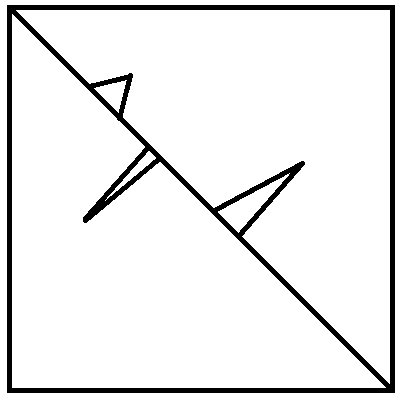
\includegraphics[width=10cm]{triangulation6}
	\centering
	\caption{Image showing an example of the third method's output}
	\label{fig:triangulation6}
\end{figure}

	The next method that was developed was an entire overhaul of the system, and this will be outlined in \ref{subsec:graphGen}



\subsection{Terrain Generation}
	To randomly generate the terrain, the Diamond-square algorithm was used. This algorithm takes four values, to be used as the corners of the terrain, and then generates the rest of the terrain. it does this by alternating between the diamond step and the square step. The algorithm is a recursive algorithm, with each iteration running on a smaller grid.
	\newline
	\par
	The Diamond-square algorithm first takes in an input, which is the size of the step taken in each iteration, to begin with this value is the size of the terrain. This value is halved at each iteration.\\

	%Running code snippet%

	The diamond steps in the algorithm are performed by iterating over all the possible y values in the grid, and at each iteration of that a for loop that iterates over all the possible x points is called. These for loops calculate every possible coordinate to perform the diamond step. The diamond step involves taking four values from the points that are at a distance of the size of the step taken away, and then averaging them and adding a random value. This step is shown in the second step and fourth step of \ref{fig:DiamondSquare}.\\

		%Diamond code snippet%

	The square step is performed by first calculating the possible values of the middle point of the squares. this is done in a for loop as the diamond step was. Then using the calculated coordinates, it will perform the square step on each coordinate. The square step involves taking the points at a distance of the size of the step taken in each of the cardinal directions. these points are then averaged and a random value is added to the value. This value is then placed in the height map at the coordinates that were found before. The square step is shown in the third and fifth step of \ref{fig:DiamondSquare}.

\begin{figure}[H]
	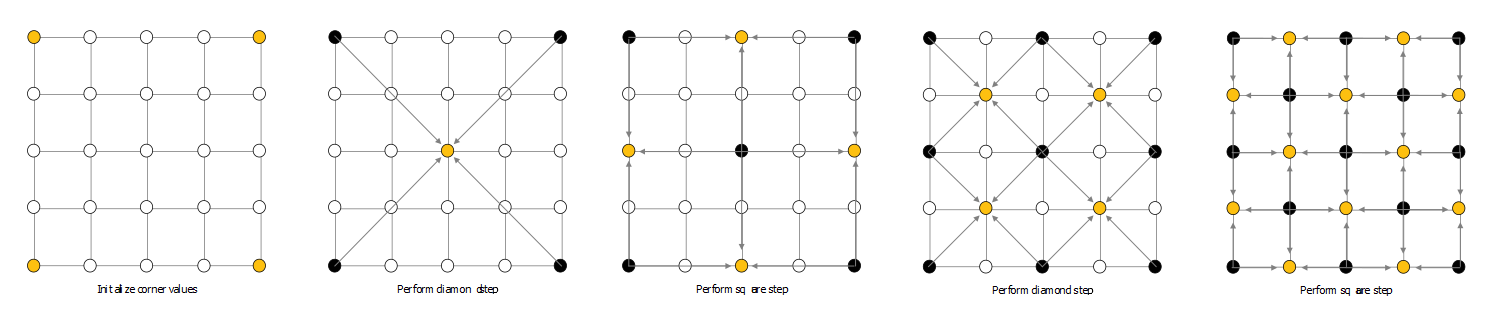
\includegraphics[width=\textwidth]{Diamond_Square}
	\centering
	\caption{Image showing the steps of the Diamond-square algorithm. Image created by Christopher Ewin.}
	\label{fig:DiamondSquare}
\end{figure}

	After the Diamond-square algorithm has been perform and has outputted the height map, the program will then use the heightmap output from the graph generation and the height map from diamond square and combine them into one height map. The equation for doing this is:\\

	$$combinedHeightMap(x, y) =  diamondSquare(x, y) - (0.05 * (1 - graphHeightMap(x, y)))$$

	This formula was determined as the graph height map needs to be subtracted from the diamond square height map in order for the rivers to show up in the terrain. The graph height map is multiplied by $0.05$ so that the rivers are not too deep on the terrain. The graph height map has to be subtracted from one as the rivers in the graph height map have the height 0, and the top of the terrain has the value of 1. This would mean if it is not subtracted from zero, the rivers would show up as mountains on the terrain.\\

\subsection{Final Terrain}
	After these steps have all been performed the program will output the terrain as a model file, as well as many text files including data about where the rivers are, where the rods should be and the route the rivers take. When the model file is imported into the game it looks like \ref{fig:finalTerrain}.

\begin{figure}[H]
	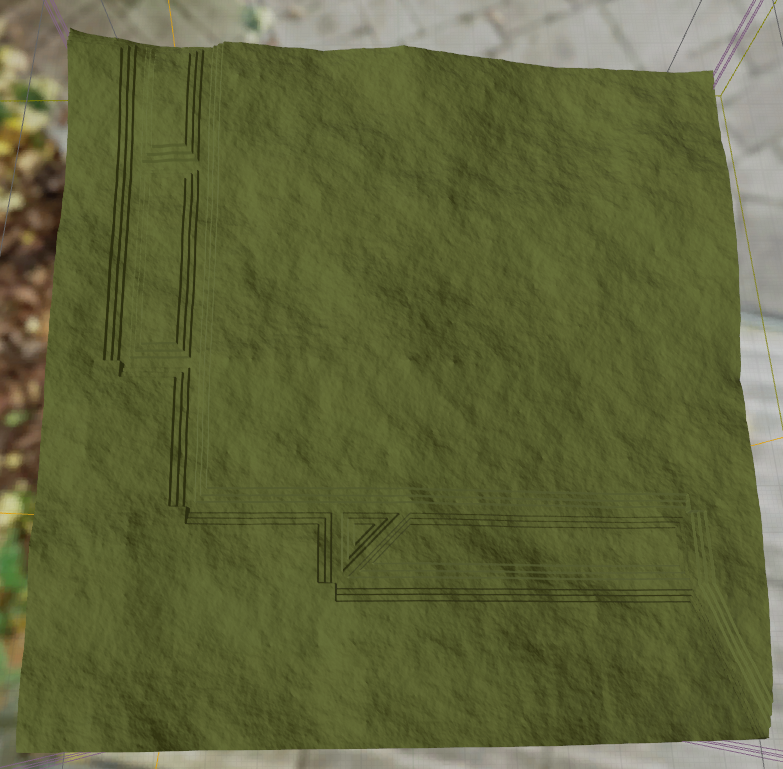
\includegraphics[width=\textwidth]{finalTerrain}
	\centering
	\caption{Image showing the final output of the terrain and river generation.}
	\label{fig:finalTerrain}
\end{figure}


\section{User Interactive Reverse Towers Of Hanoi}
The logic for the reverse Towers of Hanoi was implemented by using collision boxes on the rod actor to act as trigger when Towers of Hanoi discs are placed and removed. This method and actor was used as the basis and control for the Towers of Hanoi logic. To differentiate between the discs, three different actors were created for each size of the Towers of Hanoi discs: small, medium and large. 
\newline
\par
A collision box covers the whole rod with a size that is bigger thane the size of the hole in each disc is set to BlockAll so a disc cannot be placed through the rod. When an actor comes in contact with the collision box, this triggers the rod actor's OnHit collision event. Within this event, it identifies the size of the actor through the name of the actor's class and does a check with the array of discs in which that specific rod currently contains. This simple check will only allow discs which are larger to be placed on top of smaller discs and also makes sure that the array doesn't add disc actors that are already in the array. When the check is passed, the collision box's collision profile name is set to OverlapAll to allow the disc that triggered the event to be placed in that rod otherwise it sets it back to BlockAll. Furthermore, it adds an upward force to the disc to show that the action the player is trying to complete is invalid. This force is only added when the player is not holding the disc to avoid issues when the player is holding the disc and are moving/looking around and accidentally touching a rod with the disc.
\newline
\par
A second collision box that is slightly larger than the first was used to handle the adding and removing of discs to the array which contains all the disc actors which the rod currently holds. When a disc overlaps this collision box it adds it to the array through the OnOverlapBegin event trigger then removes it from the array with the OnOverlapEnd event trigger. When a disc is added to the array, it sets all the discs below it to not allow the player to grab it. This is done to keep with the Towers of Hanoi logic of only the disc at the top of stack being movable.
\newline
\par
A bonus feature to help with placing the discs was implemented with the `snap to rod' feature. When a disc is allowed to be placed on the rod so the disc is larger than the disc below it, then as soon as the OnOverlapBegin collision event is triggered, the disc is teleported to the top of the rod with its rotation reset so it can slide down the rod. This is useful as it can sometimes be bothersome to the player to place the disc exactly so the rod can fit exactly through the hole of the disc. This feature is only in effect when the disc is not currently being held by the player to avoid the disc teleporting whilst the player is still holding the disc which causes the disc to still be attached to the player's hand even though the disc is not in range of the hand's grab sphere.

\section{River Graph Flow}
Graph flow logic was implemented by using information generated with the terrain such as the nodes, IDs of rivers and knowing which rivers are connected to which. An actor for each river is created with a mesh using the UProceduralMeshComponent and the vertices supplied in the rivers.txt file. Each river is given an ID with the first part of the 2 numbers of the ID as the node the river is connected to and the last two numbers as the other node the other end of the river is connected to. This means that a series of river connections have the last two numbers of a river ID identical to the first two numbers of the next river in the connection.
\newline
\par
The river actors are placed in the game world by transforming the coordinates of the vertices for the river mesh generation. Since the coordinate system used for the terrain generation is different to the one used by the Unreal Engine, coordinates produced needs to be transformed so they are correctly placed in the game world as seen in Figure \ref{fig:coordinatesystem}. The X axis is shown in red, Y in green and Z in blue. The top shows the difference in coordinate systems with the coordinate system used to generate the terrain and its output on the left and the Unreal coordinate system on the right. The bottom shows a top view of the terrain ignoring the Z axis since it is the same for both coordinate systems. (0,0) for the terrain file starts at the top left corner where as in Unreal the terrain mesh is placed at the middle of the world at (0, 0, 0). It shows an example of a terrain size used of (1024, 1024) and since the terrain mesh is placed at (0, 0) in Unreal, the centre of terrain becomes (0, 0).
\newline
\par

\begin{figure}[H]
	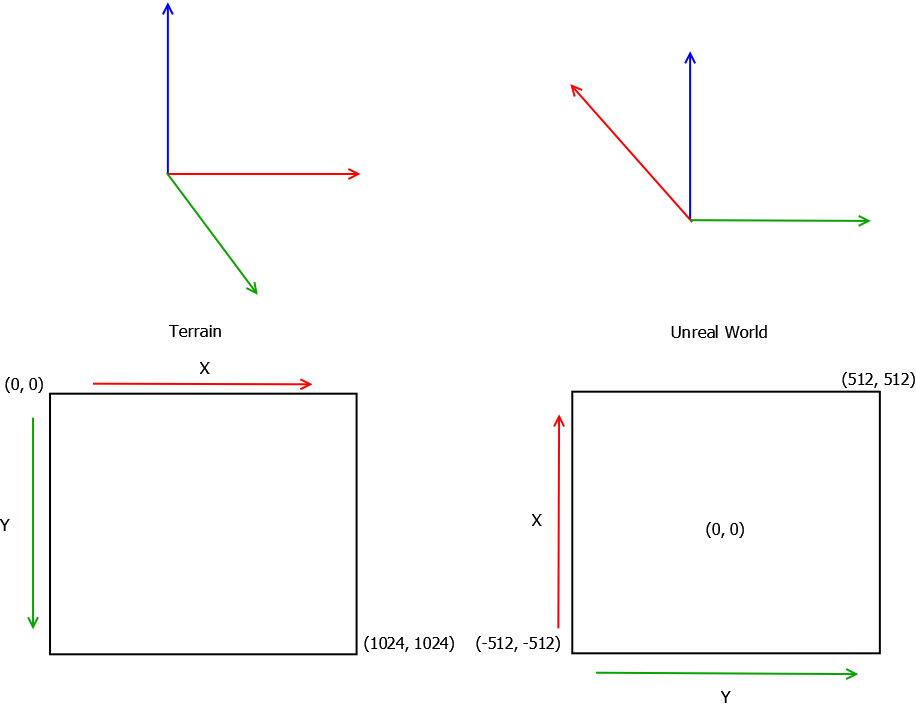
\includegraphics[width=\textwidth]{coordtransform}
	\centering
	\caption{Image showing how terrain coordinates are different to Unreal Engine coordinate system}
	\label{fig:coordinatesystem}
\end{figure}

To calculate the transformation, a bounding box surrounding the terrain mesh is created as seen in Figure \ref{fig:boundingbox}. The vertices of this box is used to compute the scale.
\newline
\par

\begin{figure}[H]
	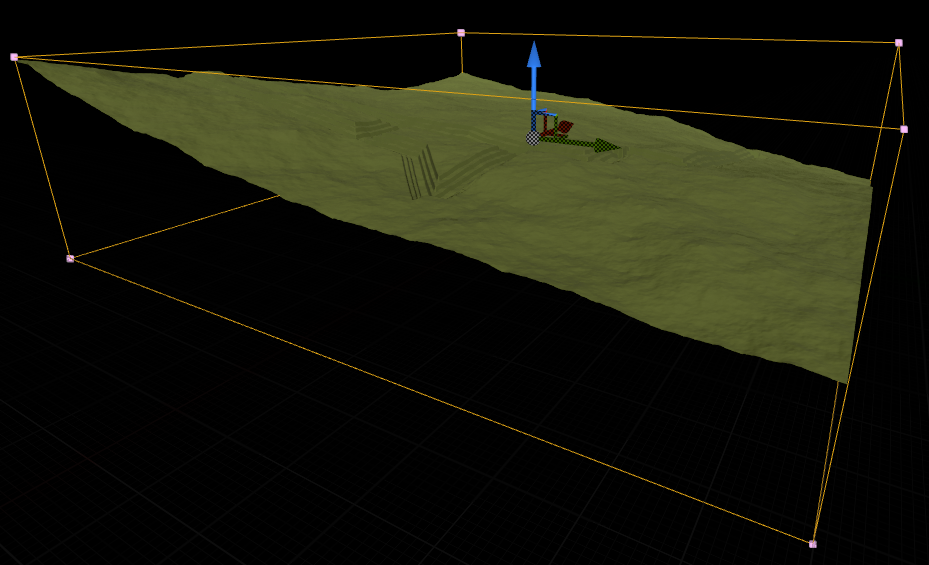
\includegraphics[width=13cm]{bounds}
	\centering
	\caption{Image showing bounding box surrounding terrain mesh}
	\label{fig:boundingbox}
\end{figure}

The following formula is then used for the X and Y coordinates since they are of the same length due to the map being square:
\[transformedCoord = (coord - \frac{1}{2}terrainMax) * \frac{worldCoordMax}{terrainMax}\]

The value of \(coord\) is the coordinate given in the output file from the terrain generation using the origin coordinate system. \(terrainMax\) is the max size of the terrain given by the terrain output so with the example in Figure \ref{fig:coordinatesystem}, this would be 1024. Half of this is subtracted as the offset to make the coordinate in the same position but instead in the bottom left corner instead of top left to fit with the coordinate system. Now this is scaled by computing the scale factor using the bounding box coordinate of a vertex but doubled as \(worldCoordMax\) to get the length of X (Y is the same) divided by \(terrainMax\).
\newline
\par
The Z transformation is similar but the only transformation needed is a scale which is just the height of the bounding box. This is computed by subtracting the Z coordinate of an upper corner of a bounding box with the Z coordinate of a lower corner. The \(terrainMax\) is not used because it would always be 1 since the Z coordinates of the terrain are between 1 and 0 with 1 as the highest point and 0 as the lowest.
\newline
\par
This method is then used to place the rods in their right places in the world so where there is a split in a river, a rod is placed on each of the rivers that branch out. The position of the rods are read in through the rods.txt file output from the terrain generation process. Each rod is given information regarding its own node ID and the river actor which it is connected to.
\newline
\par
The source of the river in the graph has a flow value hard coded and then iterates through its river connection changing the flow value of each river then when it reaches the final river it means that the river has reached a node where it splits in to two. This split has a rod for each river in order for the player to change the flow of each river. With rods with no discs, the flow value is just split simply in half between the two rivers which then follows the same procedure as before and changes the flow value of the rivers in its river connections.
\newline
\par
With the case of rods with discs in them, the flow is then affected depending on which discs are used. A small disc will reduce the flow value of the river by a \(\frac{1}{6}\), medium disc by \(\frac{1}{3}\) and a large disc by \(\frac{1}{2}\). This means using all three discs would reduce the flow to 0 so completely blocking it off. Adding or removing a disc from a rod would change the flow value for the river the rod is connected to which then changes the flow value of all the rivers that this river affects.
\newline
\par
In order for the player to easily distinguish a difference in the flow of a river when changing them with the discs, the opacity of the material used on the river will change depending on the flow value as a percentage of the original flow value at the source.

\section{Flow Dependant Flora}
Flower models are spawned around each of the nodes with rods. Flower model is royalty free and taken from cgtrader\cite{flowermodel}. The first node with rods do not have flowers as the flows of the river that will act as input to this node are the same value as the flow at the source due to the fact that it has yet to be split. These flowers will act as indicators to the player whether or not they are getting closer to the goal.
\newline
\par
The position of the flower models are computed by using the coordinates of the nodes found in the nodes.txt file output through the terrain generation procedure. The coordinates are then transformed to be placed correctly in the world with the same process as before. Another file is used called nodeConnections.txt which shows information on directions of the rivers that node is connected to. This is used to place the flowers in places on the terrain where there is no river. Due to method used to generate the terrain a river can go in one direction out of a possible 8. These possible directions can be described using the points in a compass e.g. North, North-East, East and so forth. Using random number generation, a flower has a one in three chance of placing a flower on a free space but makes sure at least one flower is placed for each node.
\newline
\par
When the player places a disc on a rod and changes the flow of the corresponding river and all the rivers affected by the change, all the river flows that serve as input in a node are accumulated and checks against the required flow to complete the goal for the node. If the flow value is over the required flow, the material for the flower petals are changed to a blue colour. If the flow value is lower than the required flow, the petals then change to a white colour. When the required flow is met, the colour is changed to an orange colour. This visual indicator helps the player see their current progress and helps to solve the puzzle.

\section{Game Goal Computation}
In order for the game to provide a challenge to players such as University of Leeds applicants during applicant days, there needs to be a goal or a puzzle to be solved. The goal is implemented using random generation every time the terrain class is added in to the Unreal Editor scene. This randomness is controlled by limiting it to only possible solutions and this is done through simulation of the game before it is created.
\newline
\par
For each rod actor in the map, one of the many possible disc combinations is chosen out of random which includes no disc on that rod. Then the game is simulated with the river flow values which are then affected by the discs on each rod. The flow value for all the rivers that act as input to the ndoes are then accumulated and is saved as the required flow for that node. The simulation is ended and resets the game with no discs on every rod then resets all the flow values to be computed again. The player will then need to try figure out the correct disc combinations for each rod through trial and error to meet all the required flows for each node to make the flower petals turn to orange which means the goal has been met. When all flowers turn to orange, the level puzzle is completed so the game transports the player to the next level.

\section{Sky Textures}
The textures for the three levels are from various places around the University of Leeds, level 1 is from in front of the Roger Stevens Building \ref{fig:level3Backdrop}, level 2 is from in front of the Great Hall \ref{fig:level2backdrop}, and level 3 is from in front of the union \ref{fig:level3Backdrop}. This was done to show that the project was developed in the University.

%Insert Images from each level showing backdrops%
\begin{figure}[H]
	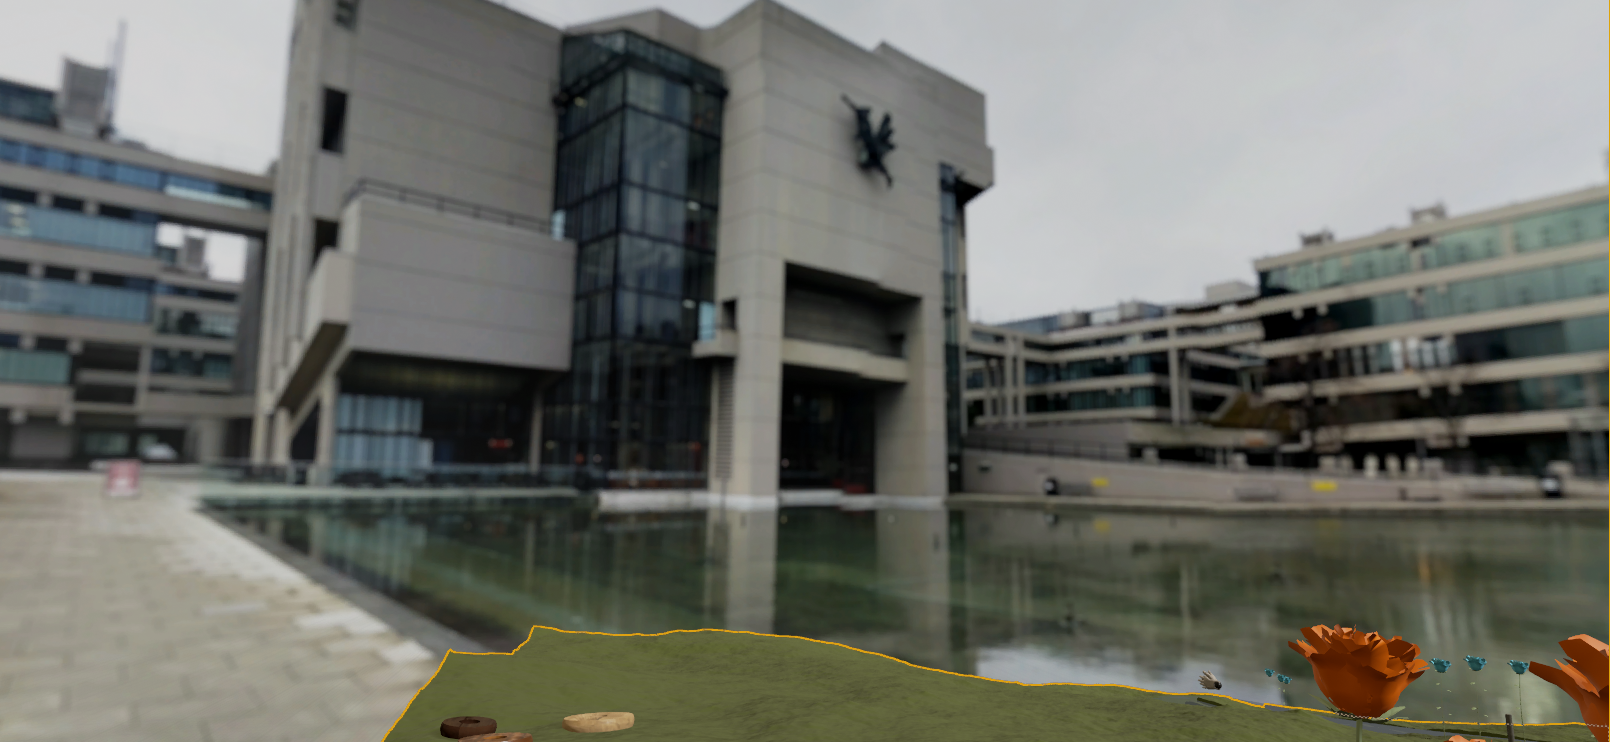
\includegraphics[width=13cm]{level1Backdrop}
	\centering
	\caption{Image showing the Sky Texture on level 2}
	\label{fig:level1Backdrop}
\end{figure}

\begin{figure}[H]
	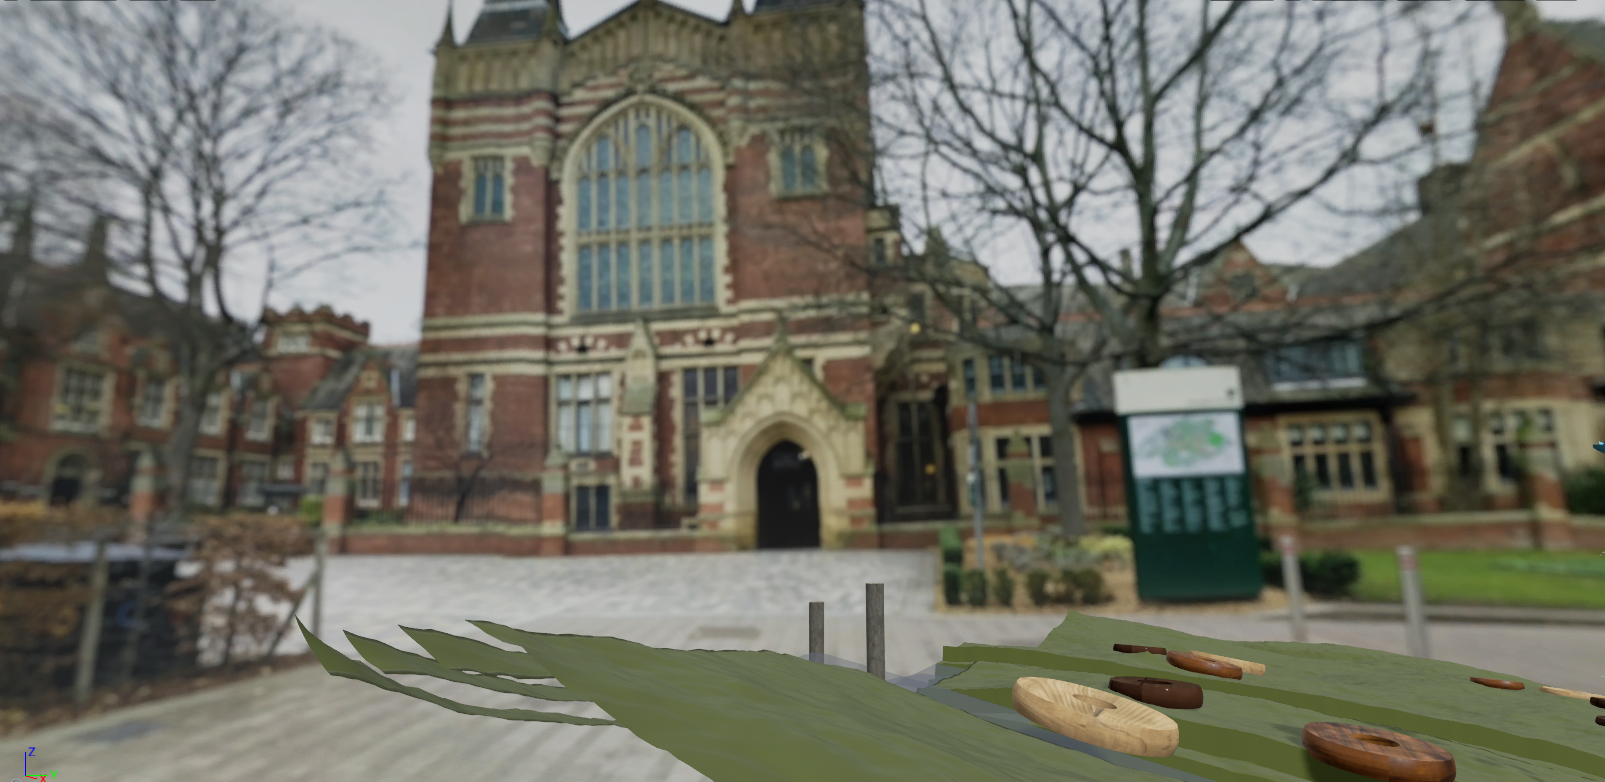
\includegraphics[width=13cm]{level2Backdrop}
	\centering
	\caption{Image showing the Sky Texture on level 2}
	\label{fig:level2Backdrop}
\end{figure}

\begin{figure}[H]
	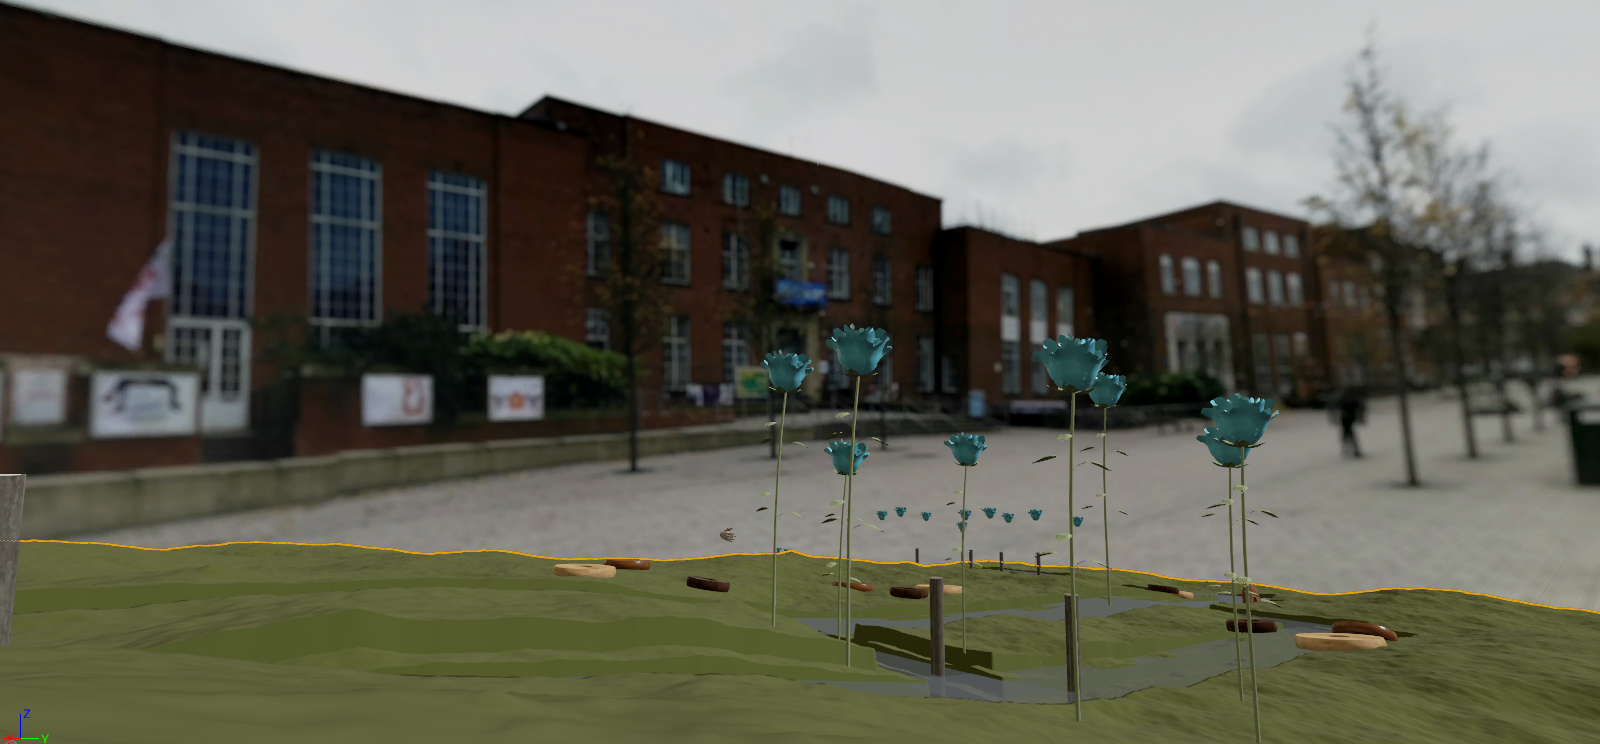
\includegraphics[width=13cm]{level3Backdrop}
	\centering
	\caption{Image showing the Sky Texture on level 2}
	\label{fig:level3Backdrop}
\end{figure}

These textures were made by first using Google's Photosphere software to create a 360 degree image of the location, this image was then flipped horizontally so that they would appear the correct way in the game. These are shown in \ref{fig:rogerStevens}, \ref{fig:greatHall}, and \ref{fig:union}. 

\begin{figure}[H]
	\includegraphics[width=13cm]{RogerStevens}
	\centering
	\caption{Image showing the 360 degree image by the Roger Stevens Building}
	\label{fig:rogerStevens}
\end{figure}

\begin{figure}[H]
	\includegraphics[width=13cm]{GreatHall}
	\centering
	\caption{Image showing the 360 degree image by the Great Hall}
	\label{fig:greatHall}
\end{figure}

\begin{figure}[H]
	\includegraphics[width=13cm]{Union}
	\centering
	\caption{Image showing the 360 degree image by the Student Union}
	\label{fig:union}
\end{figure}

These images were then separated into six images using a blender file obtained from "Aerotwist.com" \cite{aerotwist}. Using these separate images they were then arranged in the order specified by Unreal in order to create a cube map using the nVidia Texture Tools \cite{unrealCubeMaps}, an example of the image ready to be exported by nVidia texture tools is shown in \ref{greatHallPre}.

\begin{figure}[H]
	\includegraphics[width=13cm]{GreatHallPre}
	\centering
	\caption{Image showing an image about to be exported by nVidia texture tools}
	\label{fig:greatHallPre}
\end{figure}

This image is then processed by nVidia Texture Tools and exported as a .dds file, a file type that is supported by Unreal Engine. This file is then imported into the Unreal project and a material is created from the file. This material is then modified slightly so that it works as a spherical texture, and then it is set as the texture for the Sky Sphere.

\section{Disc Respawning}
An issue that was found during testing was that the discs could easily fall off the terrain. This was solved by placing invisible walls around the terrain, which stopped the discs from flying off of the edge of the terrain as they would just bounce off the wall. This wall could not be too close to the terrain however, as sometimes the discs would need to be placed on the edges of the terrain as a rod would be close to the edge of the terrain. This meant in addition to the invisible wall around the terrain, a trigger box had to be added underneath the terrain. A trigger box is an object in the world that when an object collides with it, it produces a collision event on the object. This was used by the discs, if the discs had a collision event caused by the trigger box, the discs would return to their original spawning location. this solved the issue of discs falling off the edge and not being to retrieve them.
\chapter{Testing and Evaluation}
\label{chapter7}

This chapter outlines how testing was conducted during the development. The overall project and solution produced was then evaluated to see if the goals created was met.

\section{Regular Testing}
Throughout the development, the demo was regularly tested. Aside from the usual testing from the members of the group during development, the weekly meetings with the supervisor provided a medium where new features implemented can be tested. Since the supervisor did not have knowledge of a feature was implemented, there was no bias in making the feature work like it was implemented. This helped with spotting bugs as the player may behave in ways that are not expected. 
\newline
\par
Also, the demo was tested with various other people such as colleagues of the supervisor. People with a range of skill level and familiarity with the hardware tested the solution produced. This provided a good insight to the accessibility of the demo with people that are not familiar with virtual reality. Some people found it difficult to get used to the unfamiliar controller and interaction whereas most people quickly learned especially with the natural grip gesture of holding a disc using the trigger button. The most important aspect that was deduced from the testing was the fact that every tester was quickly immersed in the world and gameplay of the demo. This meant that the world created was interesting and the gameplay aspect of it added to their enjoyability as goal was set for them to complete.
\newline
\par
In summary with the regular testing conducted, it demonstrated that demo created is interesting and immersive to people. The virtual world the player is in helps them experience the capabilities of virtual reality and the added game goal gave the player to opportunity to navigate the world and complete the level. The pitfall of the demo was that the player had to be briefed before hand on the controls and game mechanic especially if they are not familiar with virtual reality. The demo was not easy enough for someone with no prior knowledge to just play. Since the demo was made for open days, this will not be a problem since someone will be there to provide the information, but a way of showing controls or game instructions in game would be an improvement that could be made.

\section{Testing Against Requirements}
	The original requirements that the client had specified were:

\begin{itemize}
	\item Create a technology demonstration for the HTC Vive
	\item Make the technology demonstration appealing to students applying to the University of Leeds.
	\item The technology demonstration has to be appealing to members of graphics industry.
\end{itemize}

	At least two out of three of these requirements have been met. A technology demonstration has been created for the HTC Vive, this has been shown and proven to the client. The technology demonstration has also been shown to be appealing to a member of the graphics industry, this was tested by showing the technology demonstration to a member from the graphics industry. The only requirement that has not been tested is if the demonstration is appealing to applying students, this has not been tested as there has been no opportunity to show the demonstration to an applying student.

	\subsection{Student Testing Plan}
		To test if the demonstration is appealing to applying students, the demonstration should be shown to ten students currently studying Computer Science at the University of Leeds, these students should ideally have varying amount of proficiency in using Virtual Reality hardware and also be from different years of the course. During the demonstration to the students several things will be noted, including how quickly they pick up on the game controls and how quickly they figure out the objective of the game. This will be used to evaluate how intuitive the demonstration is. This is important to know as if it is not intuitive enough, then a small explanation will need to be added to the game, either as a small text introduction, or a person telling the students how to play. After the student has completed the demonstration they will be asked to take a small survey containing questions about what they thought about the demonstration, and if they were shown this on an open day would they have a higher chance of picking the University. If most of the surveys contain positive responses, then the demonstration has passed that requirement.

\section{Client Evaluation}
	The client has been shown the technology demonstration and is pleased with how the demonstration has progressed. The client was shown a final version of the product and had no major criticism about the demonstration. It was demonstrated that all features and tasks that was set out to be completed was met with a few extra features such as the campus skyboxes.

\section{Project Evaluation}
\subsection{Schedule}
	For this project the schedule was fairly accurate in terms of how long everything would take to do. There were three separate occasions when the schedule was not held to, but the project was back on track the week after. These three occasions were:
	\begin{itemize}
		\item The Virtual Reality features were not done by the week that they were supposed to be done. This was due to the fact that there was no room for the Vive to be set up in, and therefore the features could not be checked as the Vive could not be used.
		\item The Tower of Hanoi logic was also not finished in the time designated by the schedule. This was due to a bug being in the code that was hard to debug.
		\item Adding water to the graph had to be delayed compared to the schedule due to the fact that the original idea we had for the water flow (placing a flat sheet of water under the graph) would not work, and a more complex solution needed to be made. The original solution did not work as each river needs to have separate flow running through it and this is not possible with all the rivers being one sheet of water. This task was pushed back further in the schedule.
	\end{itemize}

	Most of the milestones for the project were met, only the first milestone was not met. This was due to the fact that a room for the Vive was not available until the week before the milestone, so the Virtual Reality features were not implemented properly.

\subsection{Additional Features}
	No additional features were implemented in the project, this was due to the fact that the baseline features were sufficiently challenging to implement, and therefore no time was available to add the additional features.

\subsection{Difficulties with the Project}
	One of the biggest difficulties with this project was the fact that only one Vive was available, and there was only one computer to develop on the Vive. This was solved by having each collaborator work on a separate part of the project, usually one would be working on the Vive using Unreal Engine, and the other would be work on the Out-of-Engine features, i.e. Randomly Generating Graphs. If the only feature that needed to be developed was in Unreal, the other member would help when a problem arises or would work on the other aspects of the project such as documentation.
	
\subsection{Meetings}
	Throughout the project we had weekly meetings with the client to discuss the progress of the project, and to show the current state of the project. These were immensely helpful to help keep the project in time with schedule, and they also helped with making sure each feature was up to the standard of the client.
	During the project the collaborators also had regular meetings in order to test the features if the demonstration, to make sure that everything worked as it should. During these meetings the collaborators would also discuss the plans for the week, and the tasks would be distributed out, and a short discussion would be had about the best way to tackle the tasks for that week.
\chapter{Conclusion}
\label{chapter8}

\section{Conclusion}
For this project, the problem that was undertaken was that the School of Computing at the University of Leeds have been using off the shelf demos for the HTC Vive virtual reality hardware. These demos are shown mainly during applicant days for potential University of Leeds students to spark interest in computing and technology. The problem was that there was no demo developed by University of Leeds students. Producing a solution for this would provide the School of Computing with software that can demonstrate what taking a computing course at University of Leeds can teach you and what the skills learnt can help you produce.
\newline
\par
In order to provide a solution, background research as well as a demo requirements investigation with the client was conducted so the problem can be specified and narrowed down to a size where the project can be undertaken within the time constraints. This consisted of brainstorming possible ideas to what the technical demo could include whilst taking in to account the limitations and requirements such as short gameplay and related to the University of Leeds. A feasibility research was also needed to make sure that all hardware and other requirements can be met for development to happen.
\newline
\par
A game was designed which included computer science aspects Towers of Hanoi and graph logic. The development of the game included random generation of terrain with randomly generated graphs as rivers using multiple algorithms such as the Diamond-square algorithm for the terrain. These are ouputted as a model file and txt files which have information where the rivers are, the nodes of the river graphs and the locations of the rods for the Towers of Hanoi logic. New terrain and river graphs can be generated easily by executing the terrain generation program again.
\newline
\par
The game portion included developing reverse Towers of Hanoi logic which means discs that larger than the discs already on the rod can be placed on top. Players have the ability to navigate around the terrain using the motion controllers to teleport and also grab the discs and drop them on the rods. River flow is affected depending on the size of the discs on the rod and how many of them there are as they are blocking the flow of the river. Flowers are placed at each node in the river with required flow values and act as visual indicators for the game progress. The player must match all the required flows for each node to make the flowers' petals orange to complete the level and advance to the next one.
\newline
\par
A skybox was created which used the Google Photo Sphere camera technology that takes multiple pictures and stitches them up to create a 360 degree picture. A cubemap was created with this to make the skybox that surrounds the player in the world. Skyboxes made with pictures taken around the University of Leeds campus was used for each of the different levels. This makes the demo meet the requirement of having the University of Leeds be part of it making it suited for demos during applicant days.
\newline
\par
With the solution produced, it was concluded that the requirements set out to meet was achieved and the problem was solved. A technical demo was designed and developed that provided a puzzle game that uses computer science concepts and included the University of Leeds. The project was a success and deadlines set in the plan were met consistently with very few minor delays.

\section{Future Work}
With the time constraint imposed, it was clear that further features could have been implemented to improve the gaming experience if more time was available and a few of these are outlined in this section.
\newline
\par
One of the improvements that could be made is to develop better loading screens to transition between each level. With the current solution, the transition between levels is made with a simple delayed fade out to black then fade in to the next level. A loading screen which congratulates the player on completing the level would help the player know that they have completed the puzzle for that level. A title/loading screen to appear at the start of the game which provides information on the game such as instructions is another improvement that could be developed. Instructions can include how the puzzle game works and what the goal is as well as information on the game controls for teleporting and grabbing.
\newline
\par
Another possible improvement is to improve the aesthetics of the game. This includes using or creating a proper water material for the rivers that is animated with river flow. The flow of the river will be more visible and a change of the flow with a disc change will be more evident to the player instead of just changing the opacity of the river material depending on the flow. Background scenery could also be improved which could be made with adding trees, plants and ambient creatures. The trees and plants can be generated using procedural generation with Lindemayer systems.
\newline
\par
Optimisations can be made to improve the performance of the game. If high resolution map sizes were generated, it has a negative affect with the game performance due to the higher number of vertices that has to be read in to Unreal and rendered. This means the map resolution is limited, so optimisng this can lead to higher resolution maps. Another optimisation that could be implemented is with the use of culling. The terrain could be split in to smaller chunks and only render the terrain chunk and actors on that chunk that the player is currently on. This could mean scaling the map to a bigger size for more complex river graphs and a larger world.
\newline
\par
A gameplay improvement that can be made is with the Towers of Hanoi discs. Currently, a set number of discs are placed around the world and the player must teleport and find these discs. This improvement is inspired by SteamVR's Vive tutorial which uses the different sections of the touchpad to spawn a different coloured balloon out of the motion controller. The game could take this idea and have the ability to spawn different sized discs using the motion controller which would make the game better for the player.

% % Maybe move to own page, as will be different for each of us?
% \section{Personal Reflection}
% \lipsum[1-1] \cite{parikh1980adaptive}

%Adds References to the table of content
%all you bibtex enteries go in the file called refs.bib
\addcontentsline{toc}{chapter}{References}
\bibliography{refs}

%any appendices you have go in a file called appendix.
\begin{appendices}
\chapter{External Material}

\section{Instruction Manual}

	This section will go over how to install the project, how to compile, how to run it and how to create a new level.

\subsection{Installing the Project}

\begin{enumerate}
	\item Download the project from GitHub. (https://github.com/kvcruzat/vivedemo)
	\item Download and install Unreal Engine. (https://www.unrealengine.com/)
	\item Launch Unreal Engine.
	\item Click the Browse button in Unreal and navigate to ~/RiversofHanoi and open RiversofHanoi.uproject
\end{enumerate}

\subsection{Compiling the Project}

\begin{enumerate}
	\item Open up Level 1 by going to File->Open Level   and then selecting Level1 under the levels directory.
	\item Make sure the terrain is in the level.
	\begin{enumerate}
	    \item If the terrain is not on the level then you must drag it in.
		\item This is done under the modes tab, that will be on the left side of the window in the default Unreal layout.
		\item Select the place tab if not selected, and then search for "Terrain Actor", this should produce one result.
		\item Drag this result into the game screen and the terrain should place itself down.
	\end{enumerate}
	\item Repeat step 2 for every level.
	\item To build the project go to File->Package Project->Windows->Windows (64-bit)
	\item Choose where the project should build to.
\end{enumerate}

\subsection{Running the Game}

\begin{enumerate}
	\item To run the game navigate to the folder that it was built to.
	\item Then there will be a file called RiversofHnaoi.exe, run this file.
\end{enumerate}

\subsection{Making a New Level}

\begin{enumerate}
	\item Navigate to ~/Randomly Generate Graphs/terrainGen
	\item Open a command line window here
	\item In the command line type "make", if no make utility is installed then install one, for example CMake (https://cmake.org/)
	\item After the project is compiled then type "graphGen.exe".
	\item This will produce the required files in ~/RiversofHanoi/Content/models
	\item To make a new level, navigate to ~/RiversofHanoi/Content/Levels
	\item Copy Level1.umap to a new file and rename it to next sequential level.
	\item Navigate to ./data and then copy and rename the folder "Level1" to the same name.
	\item Navigate to ~/RiversofHanoi/Content/models and copy the following files
	\begin{itemize}
		\item connections.txt
		\item nodeConnections.txt
		\item nodes.txt
		\item rivers.txt
		\item rodIndex.txt
		\item rods.txt
		\item terrain.m
	\end{itemize}
	\item Move these files to ~/RiversofHanoi/Content/Levels/data/levelx, where x is the number that it was renamed to before.
	\item Open the level in Unreal Engine by going to File->Open Level and selecting the new level.
	\item Check so that everything looks right and that the terrain model is in the game.
\end{enumerate}


\chapter{Ethical Issues Addressed}
There were no ethical issues to address.
\end{appendices}
\end{document}